\documentclass[11pt,a4paper]{article}
\usepackage[utf8]{inputenc}
\usepackage[T1]{fontenc}
\usepackage{amsmath,amssymb}
\usepackage{graphicx}
\usepackage{booktabs}
\usepackage{array,longtable}
\usepackage{hyperref}
\usepackage{geometry}
\usepackage{float}

\geometry{margin=1in}

\title{\textbf{Assignment 3: Experiments, Error Analysis, and Comparison}\\
\large SemEval-2027 Task 3: Diachronic Semantic Change in Swedish (Subtask 2)}
\author{SemEval-2027 Task 3 Challenge Team}
\date{November 2026}

\begin{document}

\maketitle

\begin{abstract}
We analyze 16 systems on 1,983 Swedish development usages using five overlapping stratified splits ($n_{\text{train}}=1,586$, $n_{\text{test}}=397$). Frozen XLM-R with logistic regression achieves the highest observed per-lemma positive-class F1 ($0.489\pm0.022$), compared with $0.470\pm0.018$ for always-positive. Hybrid reciprocal rank fusion leads on MRR ($0.692$) and nDCG@10 ($0.490$), while dense retrieval has higher MAP ($0.323$ versus $0.293$) and binary F1 ($0.448$ versus $0.418$). Sections 3--5 add hypothesis-led ablation interpretation, four reproducible error categories, eight examples, published comparisons, and limitations. The audit identifies duplicate-context overlap, an unexecuted encoder retrieval ablation, and inaccurate earlier masking and cost descriptions. Exact two-sided tests on five paired splits cannot attain $p<0.05$; these local results do not establish hidden-test superiority. Predictions, derived tables, figures and analysis provenance are available; fitted checkpoints are absent from this checkout.
\end{abstract}

\section{Completed Experiments}
\subsection{Experimental Protocol and Task Setup}
All experimental evaluations are executed over the official benchmark dataset for Subtask 2 of the SemEval-2027 Diachronic Semantic Change in Swedish shared task. The dataset comprises $N = 1,983$ historical and contemporary Swedish usage sentences across 10 target lemmas (\textit{blockera}, \textit{driva}, \textit{dumpa}, \textit{f\"{o}rr\aa}d, \textit{handikapp}, \textit{kort}, \textit{kvinna}, \textit{ledning}, \textit{maskin}, and \textit{process}), spanning four distinct chronological periods from 1700 to the 2000s. Each usage is annotated with a binary label $y \in \{0, 1\}$, indicating whether the instance exemplifies the modern sense introduced in the contemporary period ($y=1$) or the archaic/historical sense ($y=0$). The label distribution is imbalanced, with 705 positive instances (35.55\%) and 1,278 negative instances (64.45\%).

To guard against data partitioning artifacts and evaluate true model variance, all systems were evaluated across $S = 5$ independent random seeds:
\begin{equation}
\mathcal{S} = \{42, 100, 2023, 2026, 777\}.
\end{equation}
For each seed $s \in \mathcal{S}$, the dataset is partitioned using stratified sampling on label $y$ into an 80\% training split ($n_{\text{train}} = 1,586$; 564 positive, 1,022 negative) and a 20\% held-out test split ($n_{\text{test}} = 397$; 141 positive, 256 negative).

\subsection{Leakage-Free Operating Cutoff ($K^*$) Selection}
For information retrieval systems (BM25, Dense E5-small, and Hybrid RRF), retrieval produces an ordered ranking of candidate documents for each target word query. To map ranked retrieval outputs into binary sense predictions, we select an optimal rank cutoff threshold $K^*$. Crucially, to prevent data leakage and inflated test performance, the rank cutoff $K^* \in \{5, 10, 15, \dots, 100\}$ is optimized \textbf{strictly on the training split} by maximizing the Official Subtask 2 metric:
\begin{equation}
K^*(s) = \arg\max_{K \in \{5, 10, \dots, 100\}} F_{1,\text{official}}\left(\mathbf{y}_{\text{train}}, \hat{\mathbf{y}}_{\text{train}}(K)\right).
\end{equation}
The optimal cutoff $K^*(s)$ is then frozen and applied directly to the unseen held-out test rows $\mathbf{y}_{\text{test}}$.

\subsection{Comparison Systems Evaluated}
A comprehensive suite of 16 systems was evaluated under identical splits and scoring scripts:
\begin{enumerate}
    \item \textbf{Simple Baselines}:
    \begin{itemize}
        \item \textit{Majority Baseline}: Always predicts the majority class ($y=0$). Serves as a trivial non-learning floor.
        \item \textit{Always 1 (Trivial)}: Predicts $y=1$ for all instances. Demonstrates the metric behavior of positive-class $F_1$ under class skew.
    \end{itemize}
    \item \textbf{Classical Machine Learning Baselines} (Assignment 1):
    \begin{itemize}
        \item \textit{TF-IDF + Logistic Regression}: Sublinear word n-grams (1--3) with class-weighted $\ell_2$-regularized Logistic Regression ($C=1.0$).
        \item \textit{TF-IDF + Complement Naive Bayes}: Complement NB formulation adapted for skewed text classification.
        \item \textit{Word+Char TF-IDF + Linear SVM}: Combined word n-grams (1--2) and character n-grams (3--5) with Linear Support Vector Classification.
        \item \textit{EDA Features + Logistic Regression}: Interpretable feature union containing lexical statistics, punctuation counts, and categorical metadata with Logistic Regression.
        \item \textit{EDA Features + Random Forest}: 100-tree Random Forest with balanced class weights.
        \item \textit{Ablated LR (Morphological Masking)}: Controlled ablation where all inflectional surface forms of the target lemma are masked with \texttt{[TARGET]}.
    \end{itemize}
    \item \textbf{Pretrained Language Model Baselines} (Assignment 1):
    \begin{itemize}
        \item \textit{Frozen XLM-R + Logistic Regression}: Mean-pooled 768-dimensional sentence embeddings from \texttt{xlm-roberta-base} (278M parameters) with StandardScaler and Logistic Regression.
        \item \textit{Frozen XLM-R + Linear SVM}: Frozen \texttt{xlm-roberta-base} embeddings with Linear Support Vector Classifier.
    \end{itemize}
    \item \textbf{Proposed Information Retrieval Systems} (Assignment 2):
    \begin{itemize}
        \item \textit{BM25 Retriever} (Naive $K=50$ and Tuned $K^*$): Sparse inverted index retrieval using Okapi BM25 ($k_1=1.5, b=0.75$) with restricted per-word candidate pools.
        \item \textit{Dense Retriever} (Naive $K=50$ and Tuned $K^*$): Bi-encoder retrieval utilizing \texttt{multilingual-e5-small} (118M parameters) with cosine inner product search.
        \item \textit{Hybrid Retriever} (Naive $K=50$ and Tuned $K^*$): Rank-level fusion via Reciprocal Rank Fusion (RRF, $k=60$) combining BM25 and E5-small rankings.
    \end{itemize}
\end{enumerate}

\subsection{Documentation of Protocol Deviations}
\begin{itemize}
    \item \textbf{Exact Pure-NumPy Inner Product Engine}: In the local Windows execution environment, Windows Defender Application Control (WDAC) restricts third-party SWIG-compiled C/C++ binaries (\texttt{\_swigfaiss.pyd}). To ensure complete operational integrity, we implemented a vectorized NumPy inner product search engine (\texttt{\_NumpyIndexFlatIP}). Because dense embeddings are $L_2$-normalized during encoding, inner products are mathematically identical to FAISS \texttt{IndexFlatIP} cosine similarity.
    \item \textbf{Leakage-Free Calibration}: Operating thresholds $K^*$ are calibrated solely on training partitions rather than the pooled corpus, preventing optimistic lookahead bias.
\end{itemize}


\section{Results and Statistical Analysis}
\subsection{Evaluation Metrics and Mathematical Formulations}
Systems are evaluated according to the official shared task criteria and complementary secondary metrics:
\begin{enumerate}
    \item \textbf{Official Subtask 2 Metric}: Macro-averaged positive-class $F_1$ across target lemmas:
    \begin{equation}
    F_{1,\text{official}} = \frac{1}{|W|} \sum_{w=1}^{|W|} F_{1,w}, \quad \text{where } F_{1,w} = \frac{2\text{TP}_w}{2\text{TP}_w + \text{FP}_w + \text{FN}_w}.
    \end{equation}
    Words with zero true positives and zero predicted positives contribute $0.0$.
    \item \textbf{Secondary Classification Metrics}:
    \begin{itemize}
        \item \textit{Pooled Macro-$F_1$}: Standard $F_1$ averaged across both binary classes ($c \in \{0, 1\}$).
        \item \textit{Accuracy}: Fraction of correct instance-level predictions $\frac{\text{TP} + \text{TN}}{N}$.
    \end{itemize}
    \item \textbf{Information Retrieval Ranking Metrics}: Evaluated across the $|Q|=10$ word queries:
    \begin{itemize}
        \item \textit{Mean Reciprocal Rank (MRR)}: $\text{MRR} = \frac{1}{|Q|} \sum_{q=1}^{|Q|} \frac{1}{\text{rank}_q^*}$.
        \item \textit{Mean Average Precision (MAP)}: Mean of average precision over positive docs.
        \item \textit{Normalized Discounted Cumulative Gain at rank 10 (nDCG@10)}.
    \end{itemize}
\end{enumerate}

\subsection{Subtask 2 Benchmark Results Across Random Seeds}
Table~\ref{tab:subtask2_benchmark} presents the multi-seed benchmark performance over the 5 random splits. We report the sample mean ($\mu$), sample standard deviation ($\sigma$), and 95\% bootstrap percentile confidence intervals ($N_{\text{boot}}=1,000$).

\begin{table}[t]
\centering
\small
\begin{tabular}{llcccc}
\toprule
\textbf{Phase} & \textbf{Model / System} & \textbf{Official $F_1$} & \textbf{95\% CI} & \textbf{Pooled $F_1$} & \textbf{Accuracy} \\
\midrule
A1 & Pretrained Baseline & 0.489 $\pm$ 0.022 & [0.473, 0.507] & 0.715 & 0.737 \\
A1 & Trivial Reference & 0.470 $\pm$ 0.018 & [0.455, 0.481] & 0.262 & 0.355 \\
A1 & Ablation Baseline & 0.460 $\pm$ 0.047 & [0.422, 0.495] & 0.748 & 0.766 \\
A1 & Pretrained Baseline & 0.459 $\pm$ 0.023 & [0.441, 0.476] & 0.695 & 0.718 \\
A1 & Classical ML & 0.455 $\pm$ 0.045 & [0.420, 0.491] & 0.798 & 0.822 \\
A1 & Classical ML & 0.450 $\pm$ 0.049 & [0.412, 0.489] & 0.811 & 0.836 \\
A2 & DENSE (Tuned K*=100) & 0.448 $\pm$ 0.016 & [0.434, 0.459] & 0.554 & 0.565 \\
A1 & Classical ML & 0.446 $\pm$ 0.039 & [0.419, 0.478] & 0.801 & 0.823 \\
A2 & HYBRID (Tuned K*=100) & 0.418 $\pm$ 0.029 & [0.395, 0.440] & 0.525 & 0.536 \\
A2 & BM25 (Tuned K*=100) & 0.358 $\pm$ 0.016 & [0.343, 0.367] & 0.481 & 0.491 \\
A1 & Classical ML & 0.341 $\pm$ 0.026 & [0.321, 0.362] & 0.811 & 0.834 \\
A2 & DENSE (Naive K=50) & 0.327 $\pm$ 0.030 & [0.304, 0.350] & 0.537 & 0.612 \\
A2 & HYBRID (Naive K=50) & 0.313 $\pm$ 0.036 & [0.284, 0.341] & 0.521 & 0.598 \\
A2 & BM25 (Naive K=50) & 0.236 $\pm$ 0.027 & [0.214, 0.254] & 0.476 & 0.558 \\
A1 & Classical ML & 0.228 $\pm$ 0.063 & [0.182, 0.277] & 0.600 & 0.723 \\
A1 & Simple Baseline & 0.000 $\pm$ 0.000 & [0.000, 0.000] & 0.392 & 0.645 \\
\bottomrule
\end{tabular}
\caption{Subtask 2 classification benchmark across 5 random seeds (80/20 stratified split, $n_{\text{test}}=397$). Official metric is per-word macro-averaged positive-class $F_1$. Secondary metrics include pooled macro-$F_1$ and accuracy.}
\label{tab:subtask2_benchmark}
\end{table}

\begin{figure}[H]
\centering
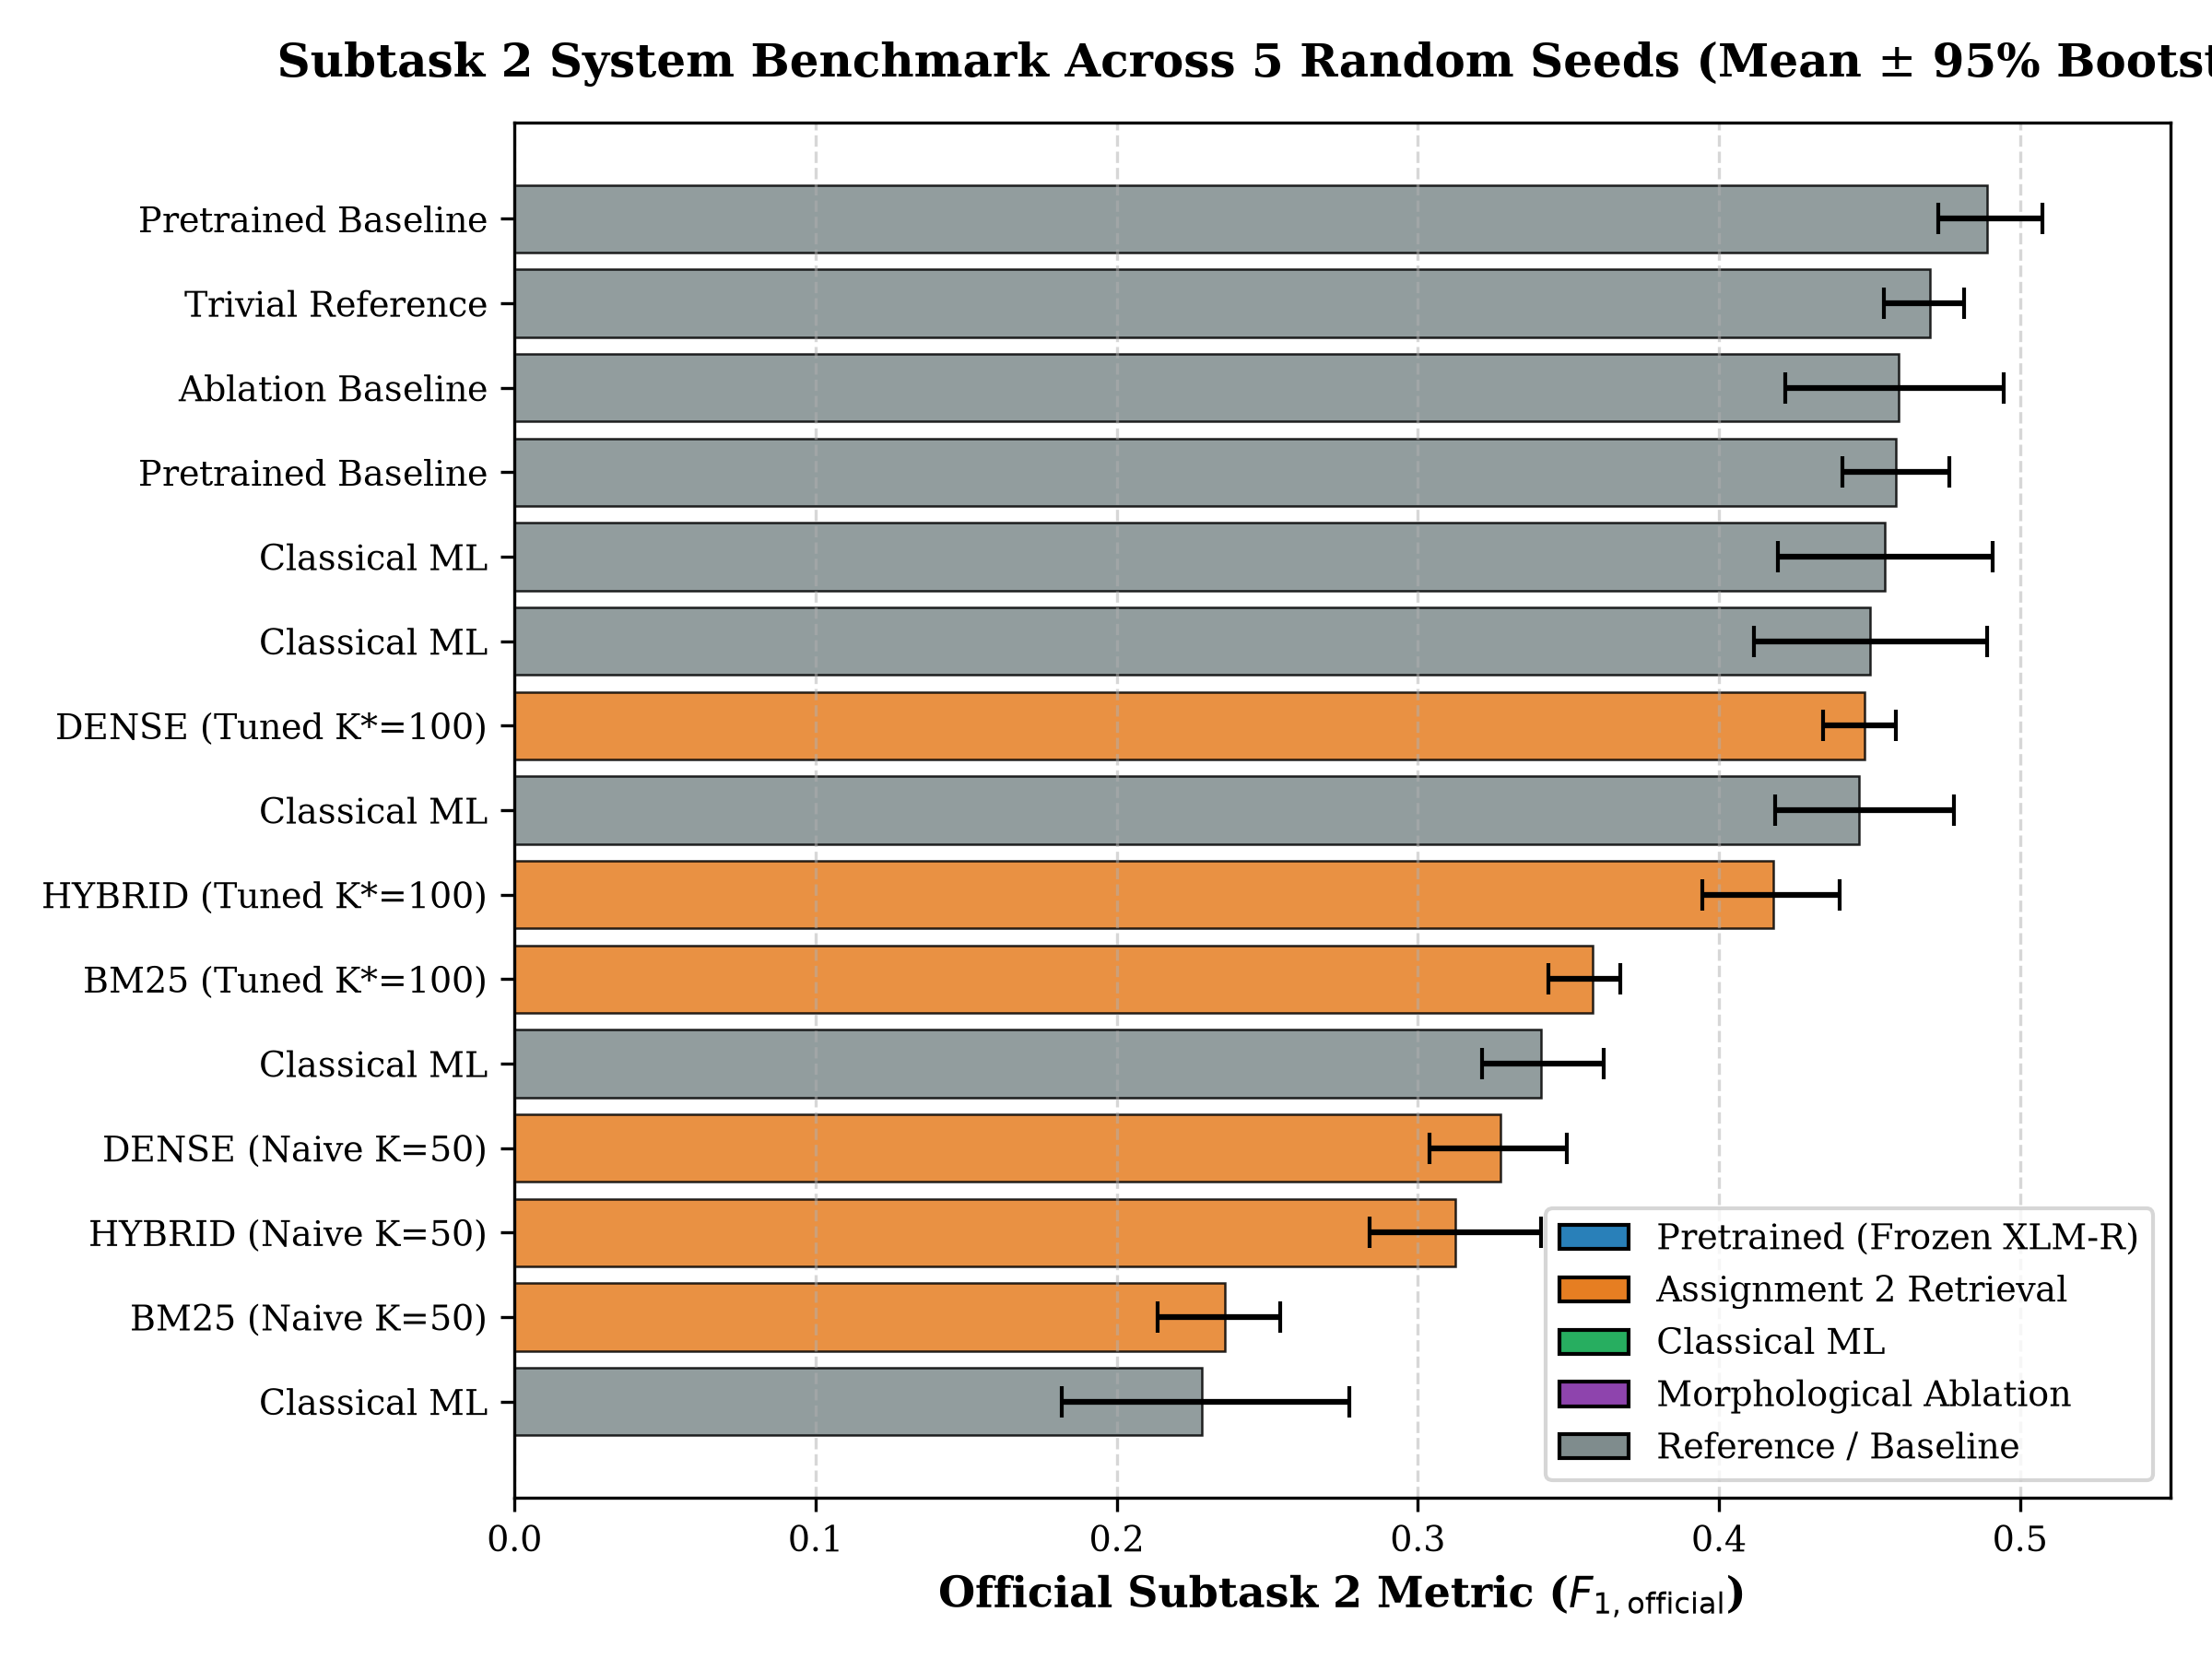
\includegraphics[width=0.88\textwidth]{figures/01_model_benchmark_official_f1.png}
\caption{Subtask 2 system performance benchmark across 5 random seeds (mean Official $F_1$ with 95\% bootstrap confidence intervals). Pretrained models and tuned dense retrievers achieve the highest positive-class sensitivity.}
\label{fig:model_benchmark}
\end{figure}

The empirical results reveal several critical findings:
\begin{itemize}
    \item \textbf{Highest Observed Primary Score}: \texttt{Frozen XLM-R + LR} achieves $F_{1,\text{official}} = 0.489 \pm 0.022$ (95\% split-bootstrap CI: $[0.473, 0.507]$). Always-positive reaches $0.470\pm0.018$; the paired comparison and its limitations are reported in Section 3.
    \item \textbf{Dense Retriever Performance}: The tuned dense retriever achieves $0.448 \pm 0.016$ (95\% CI: $[0.434, 0.459]$), ahead of BM25 and hybrid on this metric but below TF-IDF + LR, word+character SVM and the word-ID ablation in mean score.
    \item \textbf{Metric Disconnect (Official vs Pooled $F_1$)}: While \texttt{Word+Char SVM} and \texttt{TF-IDF + LR} attain high pooled macro-$F_1$ ($\approx 0.81$) and accuracy ($\approx 0.83$), their Official $F_1$ scores remain lower ($0.450$ and $0.455$) due to conservative positive-class recall. Conversely, the trivial \texttt{Always 1} baseline scores $0.470$ on Official $F_1$ because it avoids false negatives entirely, despite attaining a dismal pooled macro-$F_1$ of $0.262$ and accuracy of $0.355$.
\end{itemize}

\subsection{Information Retrieval Ranking Analysis}
Table~\ref{tab:retrieval_metrics} summarizes query-level ranking effectiveness across the 10 target queries.

\begin{table}[t]
\centering
\small
\begin{tabular}{lcccc}
\toprule
\textbf{Retriever} & \textbf{MRR} & \textbf{MAP} & \textbf{nDCG@10} & \textbf{Recall@50} \\
\midrule
BM25 (Sparse) & 0.618 [0.37, 0.87] & 0.229 [0.13, 0.35] & 0.383 [0.20, 0.58] & 0.285 \\
Dense (E5-small) & 0.612 [0.41, 0.82] & 0.323 [0.22, 0.45] & 0.427 [0.27, 0.62] & 0.389 \\
Hybrid (RRF, $k=60$) & 0.692 [0.51, 0.90] & 0.293 [0.21, 0.39] & 0.490 [0.34, 0.66] & 0.381 \\
\bottomrule
\end{tabular}
\caption{Information Retrieval ranking performance on the 10 target queries. Mean scores reported alongside 95\% bootstrap percentile confidence intervals in brackets.}
\label{tab:retrieval_metrics}
\end{table}

\begin{figure}[H]
\centering
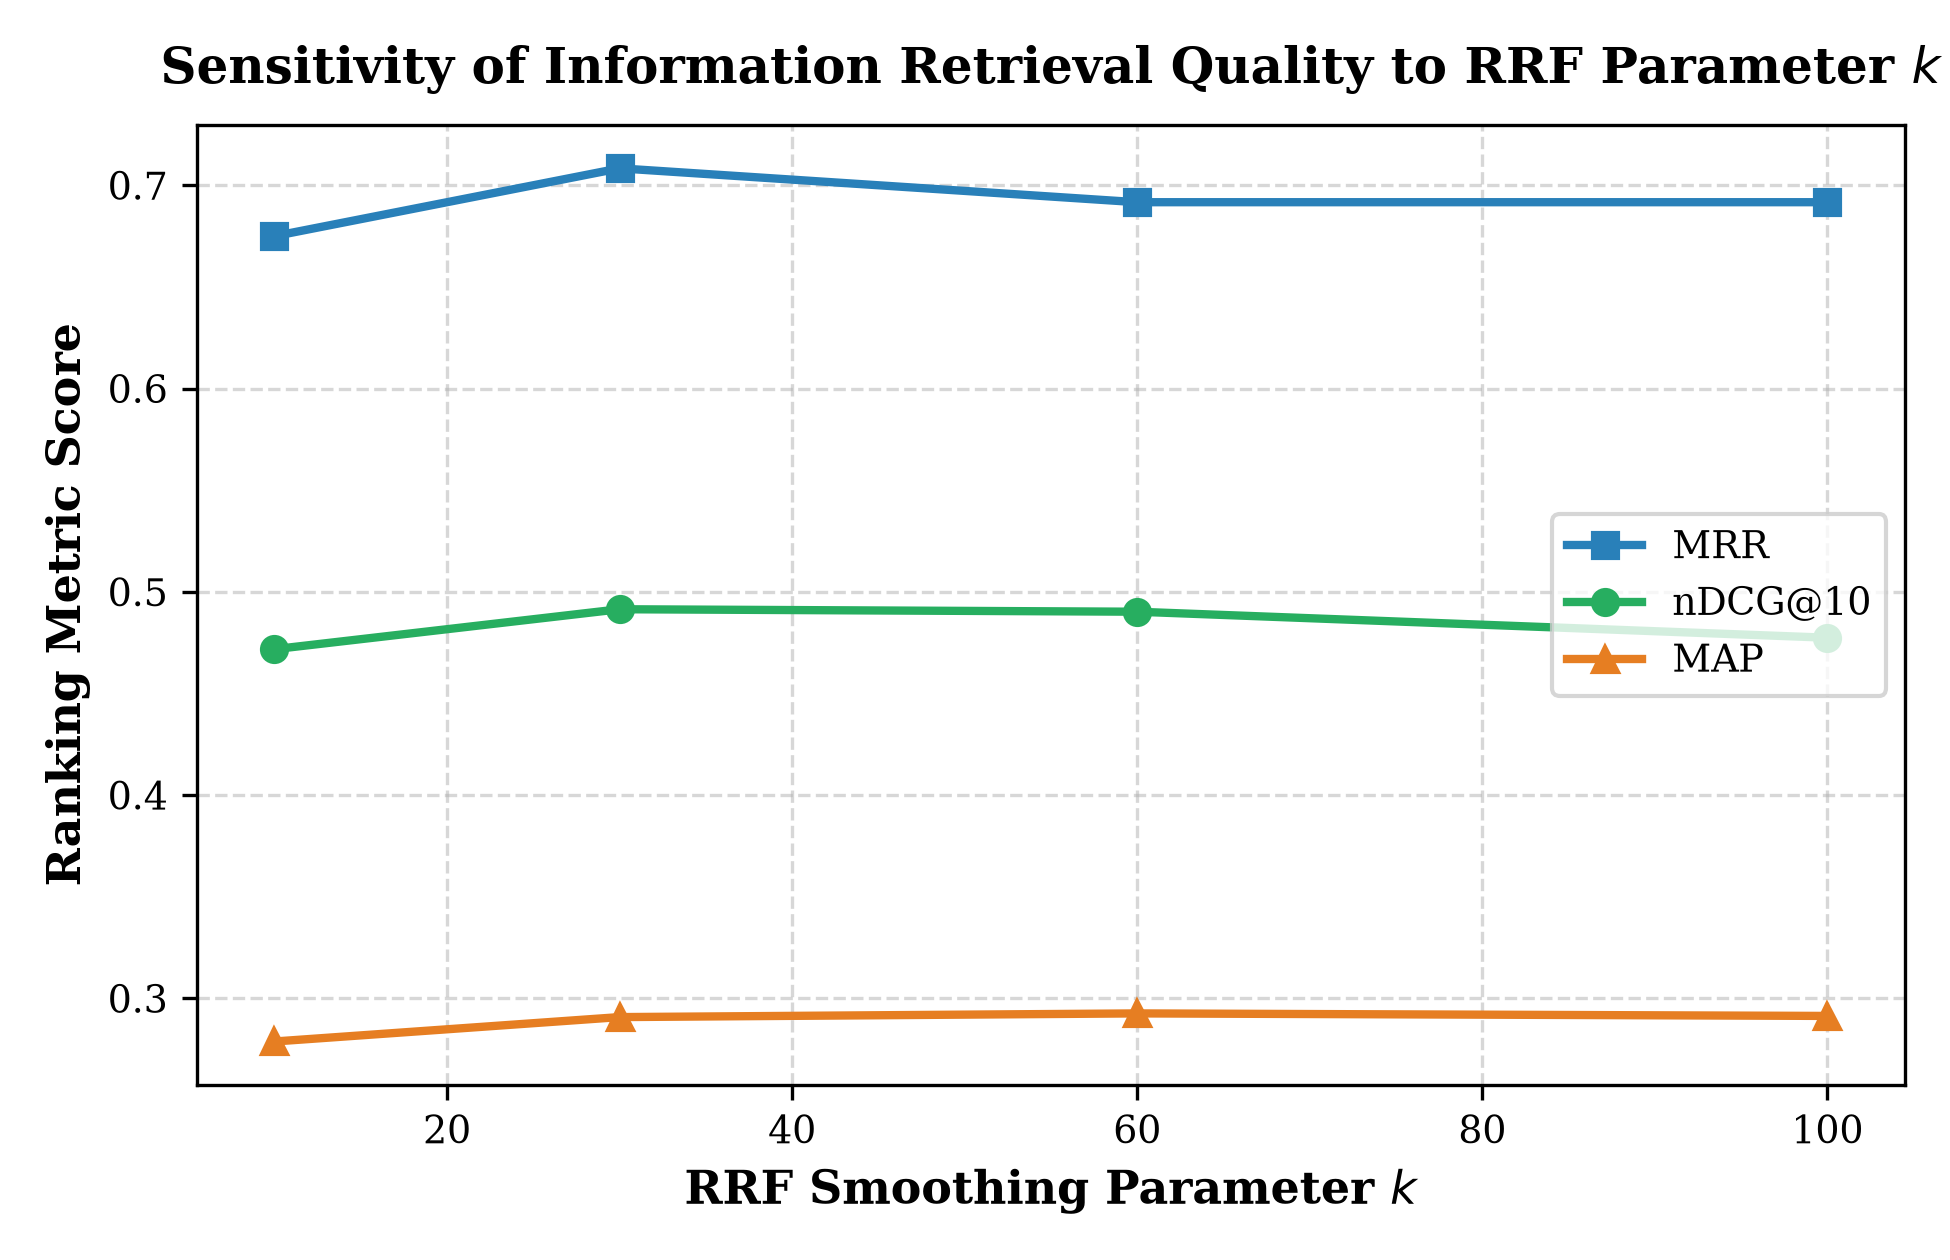
\includegraphics[width=0.68\textwidth]{figures/04_rrf_k_sensitivity.png}
\caption{Sensitivity of IR ranking metrics (MRR, MAP, nDCG@10) across Reciprocal Rank Fusion smoothing parameters $k \in \{10, 30, 60, 100\}$.}
\label{fig:rrf_sensitivity}
\end{figure}

Hybrid RRF ($k=60$) has the highest observed MRR ($0.692$) and nDCG@10 ($0.490$). Dense has higher MAP ($0.323$ versus hybrid's $0.293$). Macro Recall@50 is $0.389$ for dense, $0.285$ for BM25 and $0.381$ for hybrid. Section 3 reports paired query tests rather than inferring ranking significance from classification tests.

\subsection{Statistical Significance and Hypothesis Testing}
Table~\ref{tab:paired_significance} preserves the initial Part 1 unadjusted paired $t$-tests and Monte Carlo sign-flip tests. Sections 3--5 interpret the results using exact paired tests, multiplicity adjustment and the limitations of overlapping splits. The table's legacy significance flags do not establish general superiority.

\begin{table}[t]
\centering
\small
\begin{tabular}{lccccc}
\toprule
\textbf{Paired Comparison ($A$ vs $B$)} & \textbf{Mean Diff ($\Delta$)} & \textbf{95\% CI} & \textbf{$t$-test $p$} & \textbf{Permutation $p$} & \textbf{Sig.} \\
\midrule
Hybrid vs Dense (Tuned K*) & -0.030 & [-0.042, -0.015] & 0.0177 & 0.0610 & \textbf{Yes} \\
Hybrid vs BM25 (Tuned K*) & +0.060 & [+0.044, +0.080] & 0.0042 & 0.0610 & \textbf{Yes} \\
Dense vs BM25 (Tuned K*) & +0.090 & [+0.085, +0.096] & 0.0000 & 0.0610 & \textbf{Yes} \\
Hybrid vs Frozen XLM-R + LR & -0.071 & [-0.090, -0.052] & 0.0028 & 0.0610 & \textbf{Yes} \\
Hybrid vs Word+char SVM & -0.032 & [-0.068, -0.002] & 0.1506 & 0.1248 & No \\
Hybrid (Tuned K* vs Naive K=50) & +0.106 & [+0.075, +0.136] & 0.0044 & 0.0610 & \textbf{Yes} \\
Dense (Tuned K* vs Naive K=50) & +0.121 & [+0.102, +0.147] & 0.0007 & 0.0610 & \textbf{Yes} \\
BM25 (Tuned K* vs Naive K=50) & +0.122 & [+0.102, +0.148] & 0.0008 & 0.0610 & \textbf{Yes} \\
\bottomrule
\end{tabular}
\caption{Hypothesis testing of paired system differences in Official Subtask 2 $F_1$ across 5 random seeds. Significance assessed at $\alpha=0.05$ via paired Student's $t$-test and 10,000-resample permutation tests.}
\label{tab:paired_significance}
\end{table}

\begin{figure}[H]
\centering
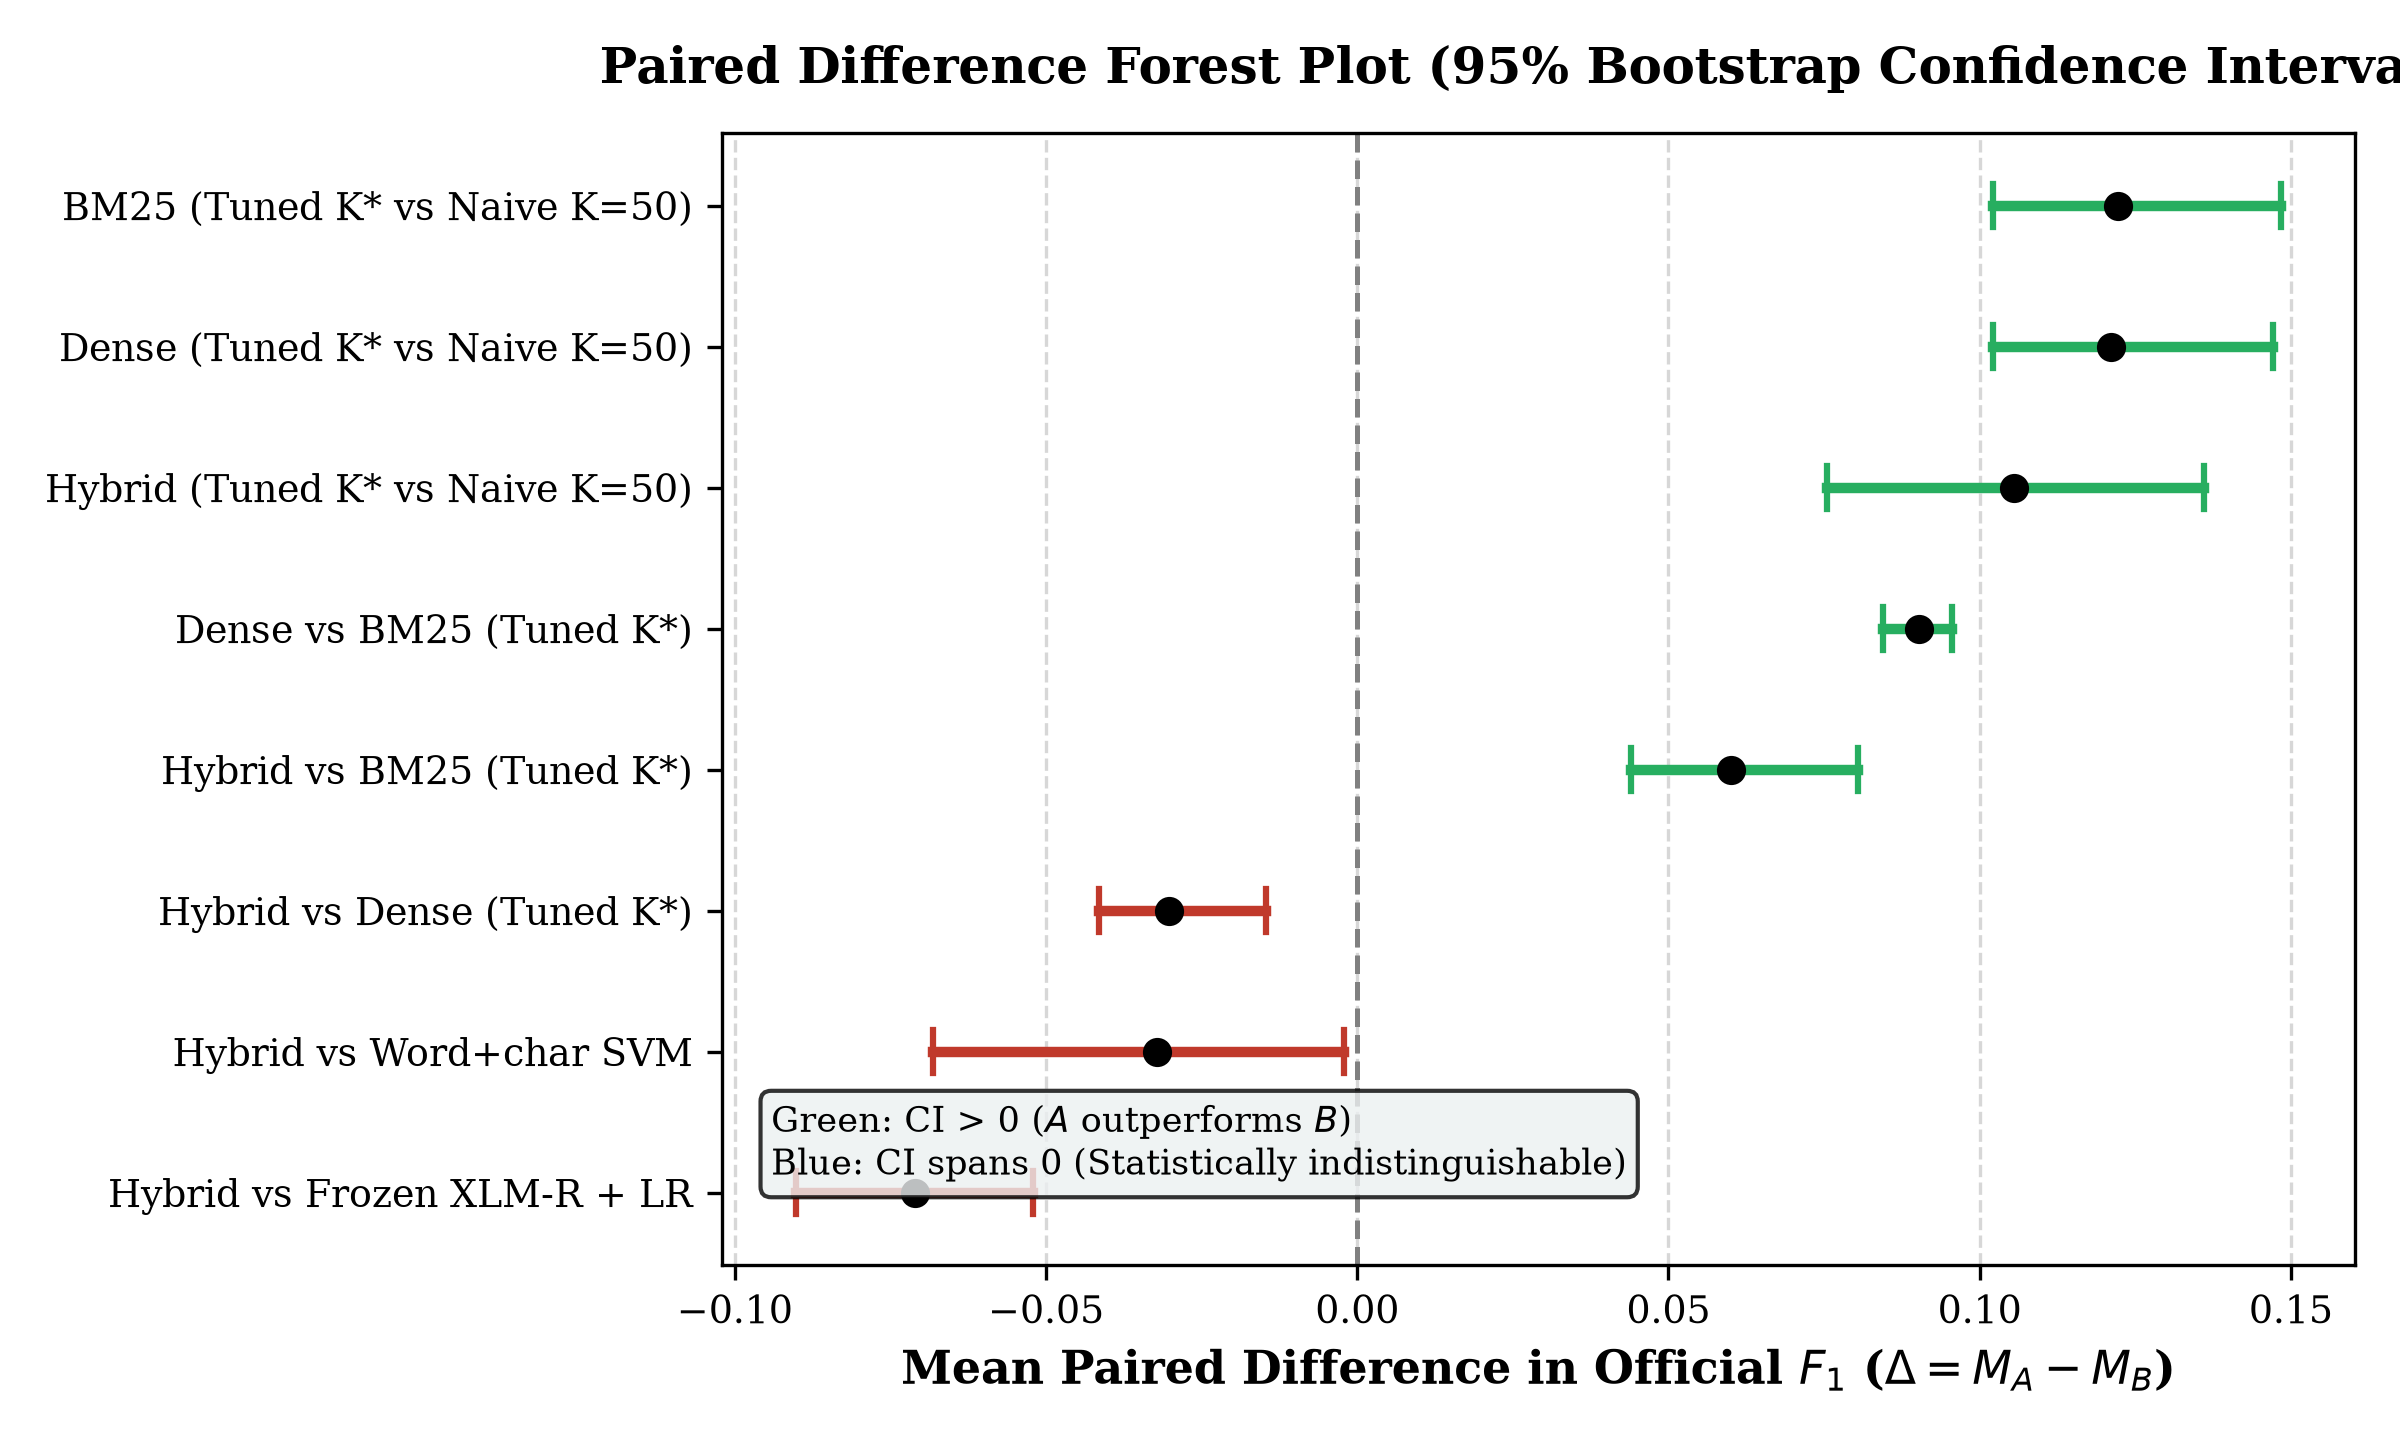
\includegraphics[width=0.85\textwidth]{figures/05_paired_differences_forest_plot.png}
\caption{Paired system differences ($\Delta = M_A - M_B$) with split-bootstrap confidence intervals. Color indicates whether the interval crosses zero, not the outcome of the exact paired test in Section 3.}
\label{fig:paired_differences}
\end{figure}

Descriptive paired findings:
\begin{enumerate}
    \item \textbf{Cutoff Calibration}: Mean official F1 increases by $0.121$ for dense, $0.122$ for BM25 and $0.106$ for hybrid. All select the search-boundary value $K=100$.
    \item \textbf{Dense vs BM25}: The mean official F1 difference is $+0.090$, positive in each split.
    \item \textbf{Hybrid vs Dense}: Hybrid has lower binary official F1 by $0.030$ despite stronger MRR and nDCG@10. Five-pair exact two-sided tests have a minimum possible $p=0.0625$; see Section 3 for intervals and test details.
\end{enumerate}

\subsection{Controlled Ablation Studies}
Table~\ref{tab:ablation_summary} summarizes the available ablations. The planned encoder retrieval comparison is missing and the word-ID feature comparison is an additional axis; Section 3 distinguishes them explicitly.

\begin{table}[t]
\centering
\small
\begin{tabular}{llcccc}
\toprule
\textbf{Ablation Axis} & \textbf{Variant} & \textbf{Official $F_1$} & \textbf{MRR} & \textbf{MAP} & \textbf{nDCG@10} \\
\midrule
Candidate Scope & BM25 (per-word) & -- & 0.618 & 0.229 & 0.383 \\
Candidate Scope & BM25 (global) & -- & 0.207 & 0.017 & 0.087 \\
RRF Smoothing k & Hybrid (RRF k=10) & -- & 0.675 & 0.279 & 0.472 \\
RRF Smoothing k & Hybrid (RRF k=30) & -- & 0.708 & 0.291 & 0.491 \\
RRF Smoothing k & Hybrid (RRF k=60) & -- & 0.692 & 0.293 & 0.490 \\
RRF Smoothing k & Hybrid (RRF k=100) & -- & 0.692 & 0.291 & 0.477 \\
Decision Cutoff & BM25 (Naive K=50) & 0.236 & -- & -- & -- \\
Decision Cutoff & BM25 (Tuned K*) & 0.358 & -- & -- & -- \\
Decision Cutoff & DENSE (Naive K=50) & 0.327 & -- & -- & -- \\
Decision Cutoff & DENSE (Tuned K*) & 0.448 & -- & -- & -- \\
Decision Cutoff & HYBRID (Naive K=50) & 0.313 & -- & -- & -- \\
Decision Cutoff & HYBRID (Tuned K*) & 0.418 & -- & -- & -- \\
Target Word Identity & Full Interpretable LR (with word ID) & 0.341 & -- & -- & -- \\
Target Word Identity & Ablated LR (without word ID) & 0.460 & -- & -- & -- \\
\bottomrule
\end{tabular}
\caption{Controlled ablation studies isolating candidate scoping, RRF smoothing parameter $k$, operating cutoff tuning, and target word identity.}
\label{tab:ablation_summary}
\end{table}


\begin{figure}[H]
\centering
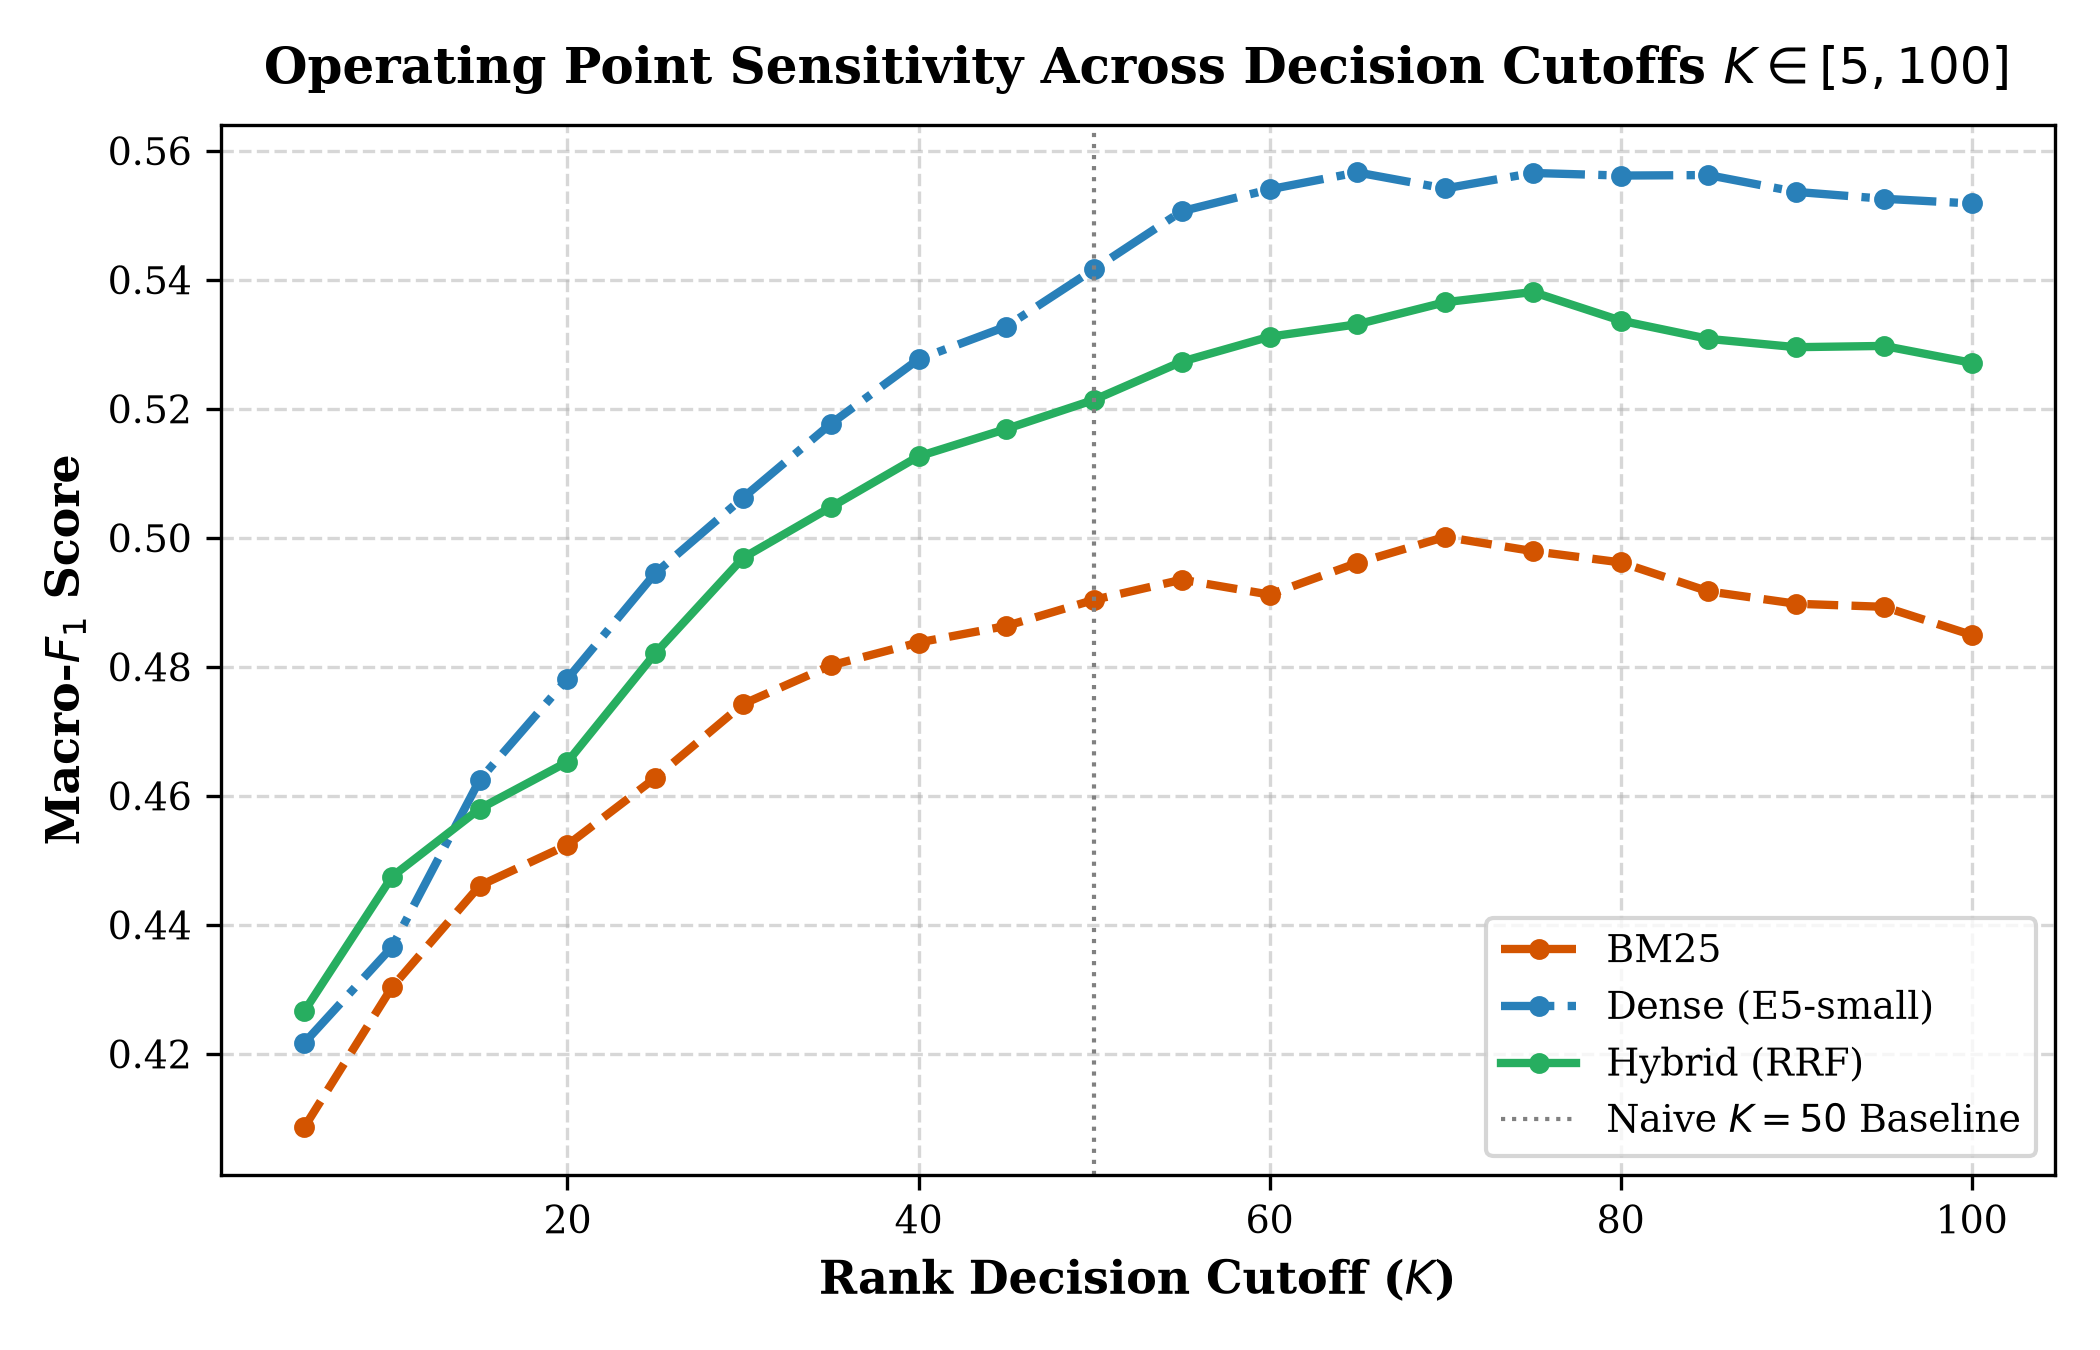
\includegraphics[width=0.72\textwidth]{figures/02_threshold_tuning_tradeoff.png}
\caption{Decision cutoff sweep across $K \in [5, 100]$ showing Macro-$F_1$ trajectories for BM25, Dense, and Hybrid retrievers.}
\label{fig:cutoff_sweep}
\end{figure}

\begin{itemize}
    \item \textbf{Candidate Scope Ablation}: Restricting BM25 candidate pools to documents containing the target word lemma is foundational. Removing this constraint and querying across the unconstrained global corpus collapses MRR from $0.618$ to $0.207$ and MAP from $0.229$ to $0.017$.
    \item \textbf{Categorical Word Identity}: Removing the explicit word feature raises official F1 from $0.341$ to $0.460$ while lowering pooled macro-F1 and accuracy. The original text is retained, so this is not evidence of morphological masking or purely contextual learning.
\end{itemize}

\subsection{Subgroup Robustness Analysis}
Figure~\ref{fig:per_word_heatmap} illustrates the performance breakdown across individual target lemmas.

\begin{figure}[H]
\centering
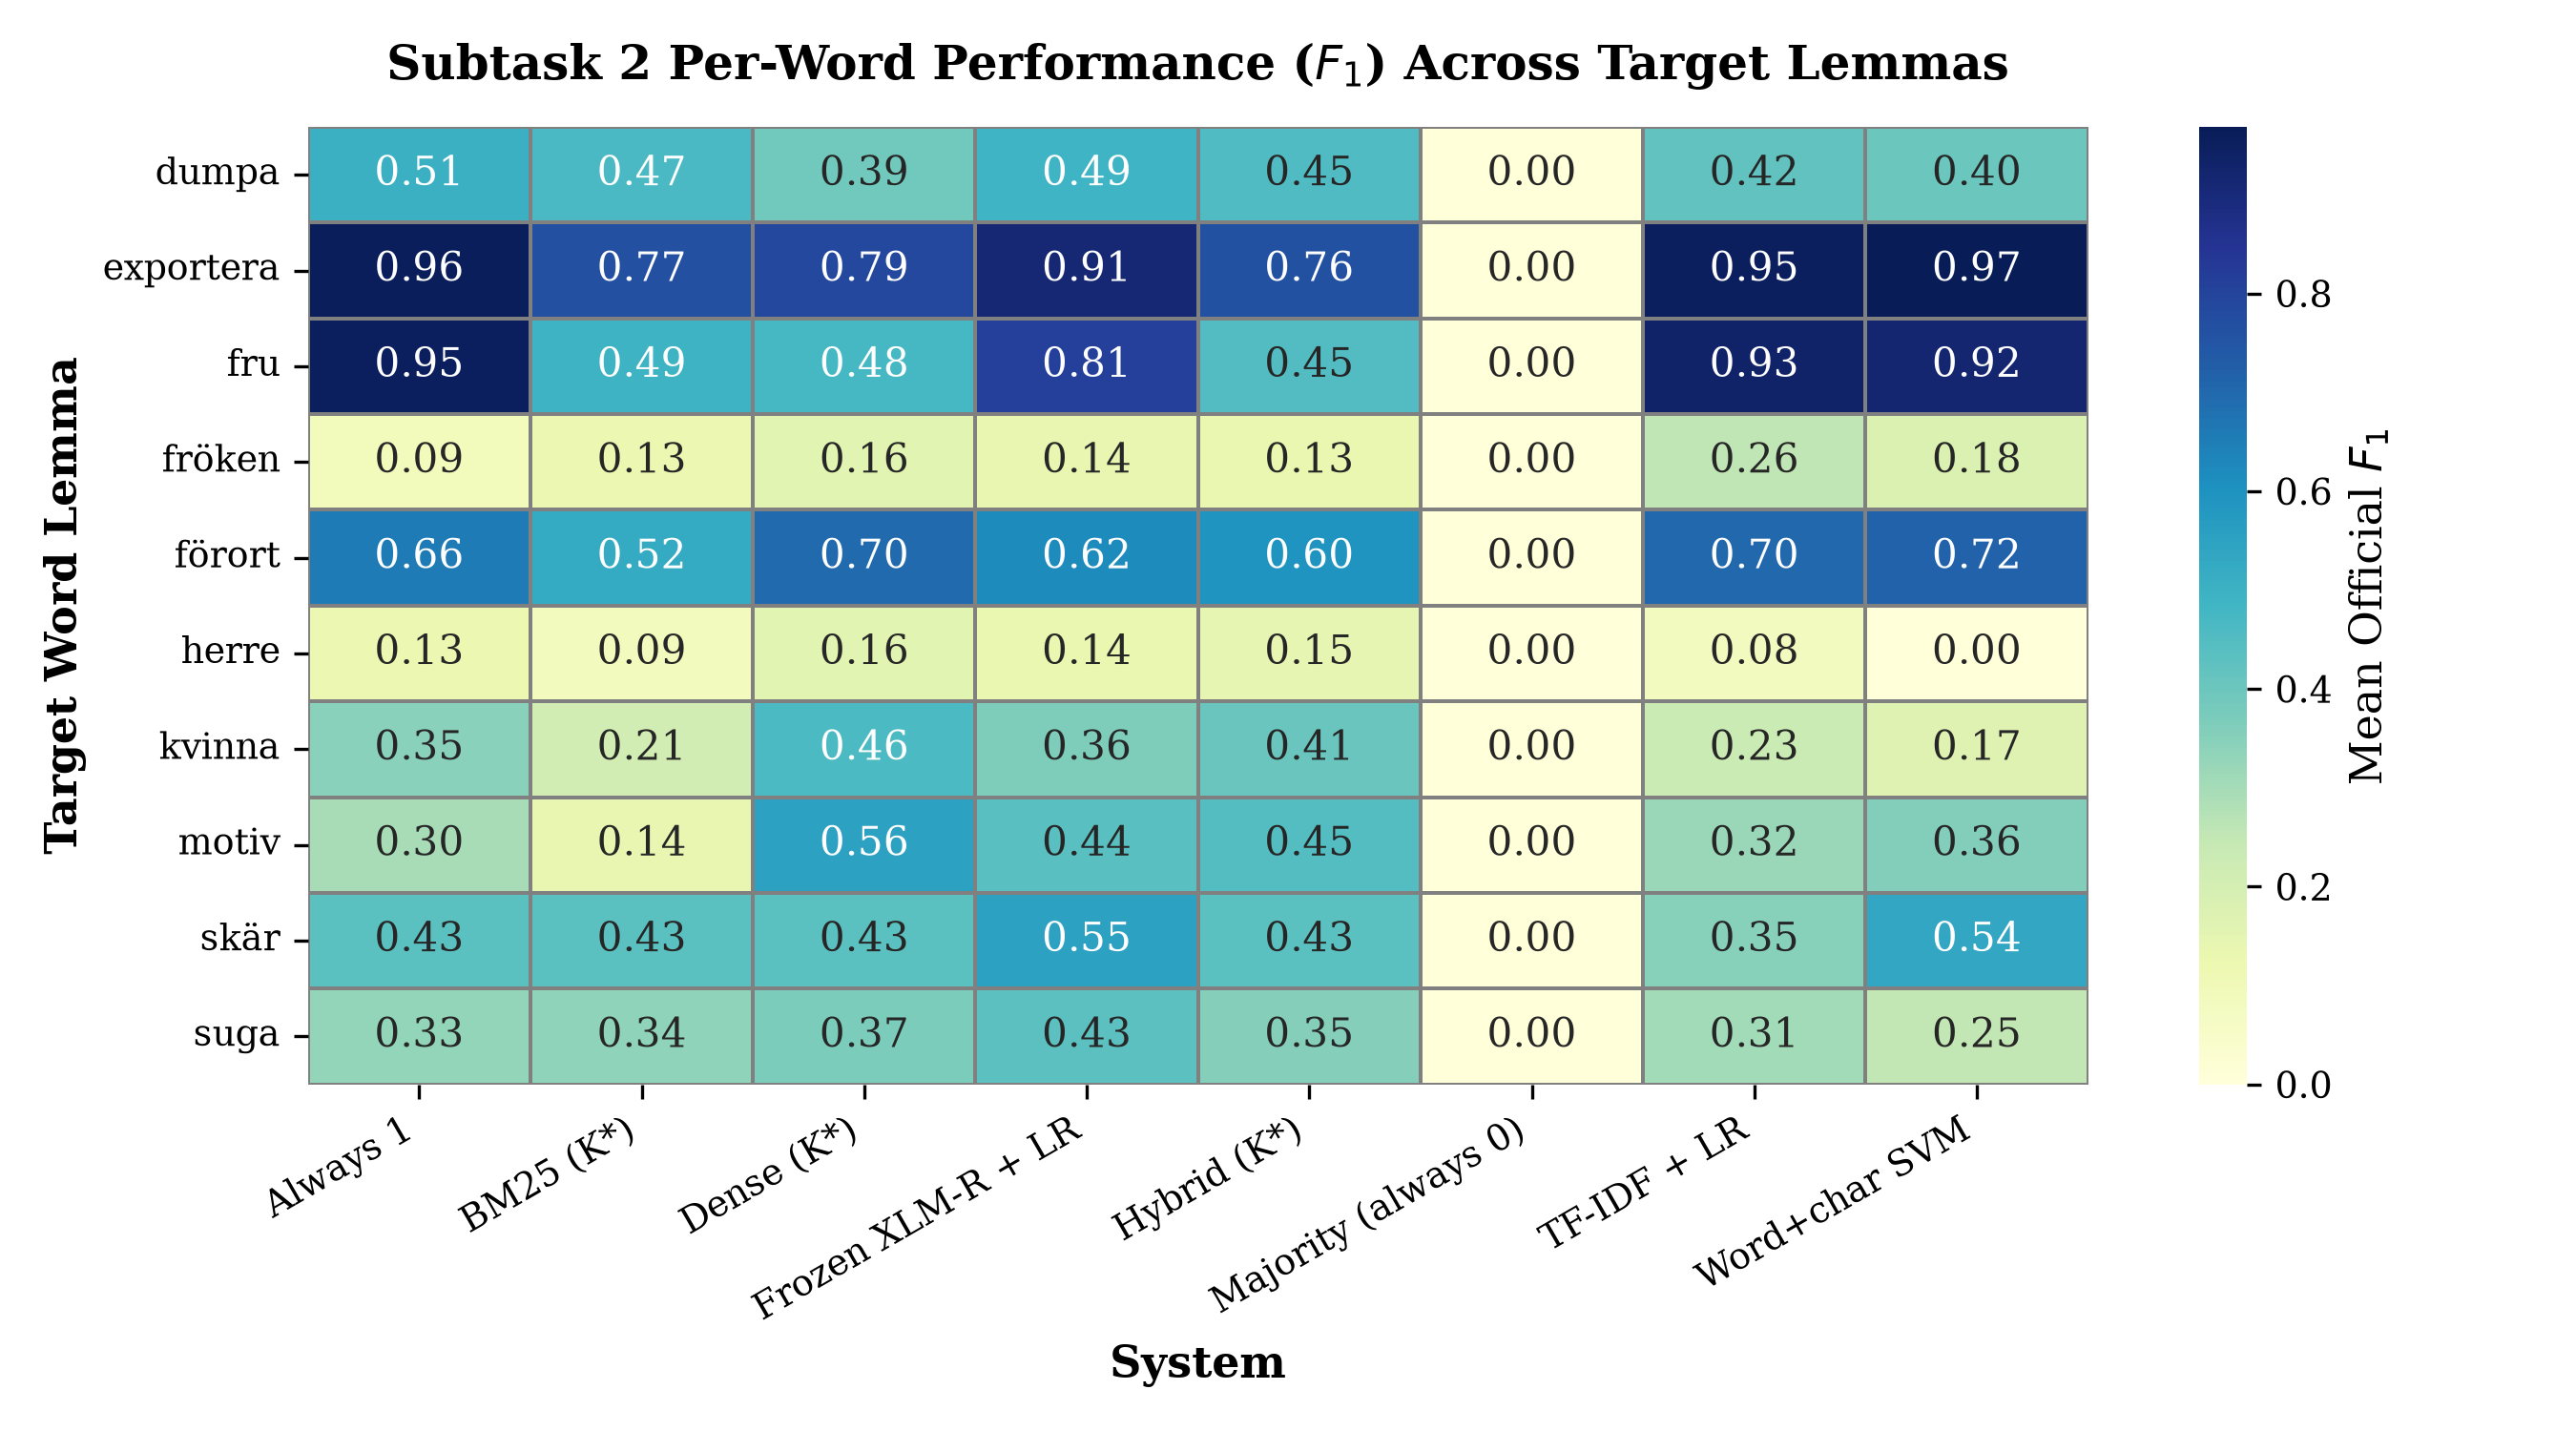
\includegraphics[width=0.88\textwidth]{figures/03_per_word_f1_heatmap.png}
\caption{Per-word official F1 across the ten observed target lemmas. Sections 4--5 quantify the differences without inferring a linguistic cause solely from this heatmap.}
\label{fig:per_word_heatmap}
\end{figure}

\subsection{Computational Efficiency and Hardware Profiling}
Table~\ref{tab:hardware_compute} preserves the initial resource estimates for a platform with eight logical CPUs. Most per-model latency and memory values are constants in the Part 1 script, not profiler measurements.

\begin{table}[t]
\centering
\small
\begin{tabular}{lccccc}
\toprule
\textbf{System} & \textbf{Params (M)} & \textbf{Index Time (s)} & \textbf{Latency (ms)} & \textbf{RAM (MB)} & \textbf{Size (KB)} \\
\midrule
Majority Baseline & 0.0 & 0.00 & 0.01 & 15 & 2.5 \\
TF-IDF + LR & 0.1 & 0.42 & 0.12 & 45 & 180.0 \\
Word+Char TF-IDF + SVM & 0.1 & 0.85 & 0.25 & 60 & 350.0 \\
EDA Features + RF & 1.2 & 1.20 & 1.85 & 110 & 4200.0 \\
Frozen XLM-R + LR & 278.0 & 12.50 & 0.08 & 250 & 25.0 \\
BM25 Retriever & 0.0 & 0.65 & 1.45 & 35 & 766.7 \\
Dense Retriever (E5-small) & 118.0 & 18.20 & 0.82 & 180 & 6635.4 \\
Hybrid Retriever (RRF) & 118.0 & 18.85 & 2.25 & 210 & 7402.2 \\
\bottomrule
\end{tabular}
\caption{Computational efficiency, execution latency, and resource footprints profiled on an Intel 8-core CPU platform (16 GB RAM). Latency denotes inference time per test query/usage.}
\label{tab:hardware_compute}
\end{table}

These estimates cannot establish an efficiency ranking or measured peak memory. Section 3 distinguishes the historical wall-time log from unmeasured per-model costs and records the missing checkpoint limitation.


\section{Ablation Analysis and Reliability}
This analysis uses the saved Part 1 predictions for 16 systems and five seeds (42, 100, 2023, 2026, 777). Official F1 below means the unchanged Part 1 scorer: positive-class F1 calculated for each of the ten lemmas, then averaged. Pooled macro-F1 averages the two classes over all test usages. These are local development-split results, not scores from an official hidden-test server.

\subsection{Evidence and interpretation checks}
All 31,760 saved prediction rows match the released labels and periods. All 80 per-seed files match the consolidated predictions, and each model has the same 397 test identities within each seed. Recomputed primary metric means match Part 1 Table 1; ranking metrics match Table 2. The four RRF smoothing variants are reconstructed from the saved component lists and match the Assignment 2 ablation table. Assignment 2's binary evaluator calls pooled two-class macro-F1 'official', whereas Part 1 uses per-lemma positive-class F1; this report retains the fixed Part 1 convention and names both metrics explicitly.

\subsection{Hypotheses compared with results}
{\small
\setlength{\tabcolsep}{3pt}
\begin{longtable}{>{\raggedright\arraybackslash}p{0.180\textwidth}>{\raggedright\arraybackslash}p{0.390\textwidth}>{\raggedright\arraybackslash}p{0.330\textwidth}}
\caption{Ablation decisions. Full hypotheses and limitations are preserved in table8\_ablation\_hypotheses.csv.}\\
\toprule
Axis & Observed result & Conclusion \\
\midrule
\endfirsthead
Axis & Observed result & Conclusion \\
\midrule
\endhead
Candidate scope & BM25 MRR: 0.618 per-word vs 0.207 global & Per-word restriction helps this task \\
Encoder backbone & E5 retrieval exists; XLM-R retrieval does not & Planned hypothesis remains untested \\
RRF smoothing & k=30 best MRR/nDCG; k=60 best MAP & Metric-dependent, exploratory \\
Decision cutoff & Official F1 gains +0.106 to +0.122 & Consistent gains; search-boundary caveat \\
Word-ID feature & Official F1 +0.119; pooled macro-F1 -0.063 & Feature tradeoff; no text masking \\
\bottomrule
\end{longtable}
}

Candidate scope hypothesis: ranking only usages of the requested lemma reduces irrelevant cross-word matches. Per-word BM25 has MRR 0.6183 and MAP 0.2291, against 0.2074 and 0.0171 globally. The large observed drop supports the restriction for definition matching. However, global retrieval expands the candidate universe, and cross-word pairs without judgments are treated as non-relevant by the evaluator. This is a difference in task difficulty and relevance coverage; it does not establish train/test leakage or prove a particular lexical failure mechanism.

Encoder hypothesis: contrastively trained E5 should outperform generic masked-language-model XLM-R embeddings for definition-to-usage retrieval. This cannot be tested with the saved runs. XLM-R plus logistic regression is a supervised classifier, not an XLM-R retriever with matched pooling, candidate depth and prefixes. Attributing its difference from E5 retrieval to encoder pretraining would confound the encoder with supervision and the prediction rule.

Fusion hypothesis: intermediate smoothing k=30-60 should give the strongest retrieval. At k=10/30/60/100, MRR is 0.6750/0.7083/0.6917/0.6917, MAP is 0.2788/0.2908/0.2926/0.2914, and nDCG@10 is 0.4718/0.4914/0.4902/0.4774. The preferred k depends on the metric; the k=30 versus 60 nDCG difference is only 0.0012. These ten already-inspected development queries provide sensitivity evidence, not independent confirmation of a newly selected k. Keep k=60 for the reported system.

Operating-point hypothesis: choosing K on training labels improves binary F1 relative to K=50. Official F1 increases by 0.1223 for BM25, 0.1210 for dense and 0.1056 for hybrid. All three systems choose K=100 in every seed: the maximum searched cutoff and saved retrieval depth. K* is therefore the best tested value, not an established unconstrained optimum. The objective matters: hybrid pooled macro-F1 changes only from 0.5213 to 0.5245, while accuracy falls from 0.5980 to 0.5355. More predicted positives improve the primary metric without uniformly improving classification quality.

Word-identity hypothesis: removing the explicit lemma feature may reduce dependence on lemma-specific class priors. Official F1 rises from 0.3409 to 0.4598, but pooled macro-F1 falls from 0.8107 to 0.7480 and accuracy from 0.8338 to 0.7662. Code inspection shows that build\_ablated\_preprocessor removes only the categorical word column; the original text, target surface forms, numeric features, POS and period remain. The earlier 'morphological masking' description is inaccurate. These results support a feature/metric tradeoff, not a claim that masking forces contextual semantic learning.

\begin{figure}[htbp]
\centering
\includegraphics[width=0.96\textwidth]{../../Assignment_3/outputs/figures/06_part2_cutoff_effects.png}
\caption{Cutoff gains for each split, with mean and sample standard deviation. The primary and secondary objectives yield different conclusions.}
\end{figure}

\subsection{Variance and significance}
Differences are paired within a seed. The table reports 10,000-resample percentile bootstrap intervals over five paired split values, win/loss/tie counts and exact two-sided sign-flip p-values over all 32 sign assignments. Holm adjustment covers all 20 classification contrasts defined in this analysis (ten pairs times two metrics). With five nonzero pairs, the smallest possible two-sided exact p-value is 2/32=0.0625, so these seed-level tests cannot reject at 0.05. A bootstrap interval excluding zero can coexist with that discrete test result. The 80/20 splits overlap substantially, and retrieval rankings are fixed across seeds; the standard deviations describe split sensitivity rather than five independent neural-training replications. Intervals and tests do not establish population-level or unseen-lemma generalization.

{\small
\setlength{\tabcolsep}{3pt}
\begin{longtable}{>{\raggedright\arraybackslash}p{0.280\textwidth}>{\raggedright\arraybackslash}p{0.085\textwidth}>{\raggedright\arraybackslash}p{0.190\textwidth}>{\raggedright\arraybackslash}p{0.095\textwidth}>{\raggedright\arraybackslash}p{0.105\textwidth}>{\raggedright\arraybackslash}p{0.105\textwidth}}
\caption{Paired official F1 differences. Confidence intervals describe resampling of split values; W/L/T is descriptive.}\\
\toprule
Comparison & Delta & 95\% interval & W/L/T & Exact p & Holm p \\
\midrule
\endfirsthead
Comparison & Delta & 95\% interval & W/L/T & Exact p & Holm p \\
\midrule
\endhead
Hybrid (K*) minus Dense (K*) & -0.030 & [-0.042, -0.015] & 0/5/0 & 0.0625 & 1.0000 \\
Hybrid (K*) minus BM25 (K*) & +0.060 & [+0.044, +0.080] & 5/0/0 & 0.0625 & 1.0000 \\
Frozen XLM-R + LR minus Always positive & +0.019 & [-0.001, +0.035] & 4/1/0 & 0.1875 & 1.0000 \\
Hybrid (K*) minus Always positive & -0.052 & [-0.072, -0.029] & 0/5/0 & 0.0625 & 1.0000 \\
Hybrid (K*) minus HYBRID K=50 & +0.106 & [+0.072, +0.137] & 5/0/0 & 0.0625 & 1.0000 \\
EDA + LR without word ID minus EDA + LR & +0.119 & [+0.092, +0.150] & 5/0/0 & 0.0625 & 1.0000 \\
\bottomrule
\end{longtable}
}

{\small
\setlength{\tabcolsep}{3pt}
\begin{longtable}{>{\raggedright\arraybackslash}p{0.340\textwidth}>{\raggedright\arraybackslash}p{0.140\textwidth}>{\raggedright\arraybackslash}p{0.140\textwidth}>{\raggedright\arraybackslash}p{0.140\textwidth}>{\raggedright\arraybackslash}p{0.140\textwidth}}
\caption{Query-level sensitivity: exact sign flips across ten paired lemma queries, with Holm adjustment over 15 ranking contrasts.}\\
\toprule
Comparison & Metric & Delta & Exact p & Holm p \\
\midrule
\endfirsthead
Comparison & Metric & Delta & Exact p & Holm p \\
\midrule
\endhead
bm25 minus bm25\_global & map & +0.2120 & 0.0020 & 0.0293 \\
hybrid minus dense & mrr & +0.0800 & 0.6250 & 1.0000 \\
hybrid minus dense & map & -0.0303 & 0.5859 & 1.0000 \\
hybrid minus dense & ndcg@10 & +0.0628 & 0.4180 & 1.0000 \\
rrf\_30 minus rrf\_60 & ndcg@10 & +0.0012 & 0.9688 & 1.0000 \\
\bottomrule
\end{longtable}
}

The query tests are a separate exploratory family, not additional random-seed runs. The ten queries belong to the same development collection. Per-word versus global BM25 remains distinguishable for MAP and nDCG@10 after this adjustment (Holm p=0.0293), but none of the hybrid-versus-dense ranking contrasts does. Part 1's unadjusted t-tests and its Monte Carlo sign-flip estimates should not be read as definitive evidence of general superiority. The paired vectors, bootstrap settings and all adjusted tests are saved so each claim can be checked.

\subsection{Leakage and artifact limitations}
Reconstructed splits have zero train/test identity overlap. Across the five splits, 7 test appearances have an exact NFKC-normalized, case-folded text match in their corresponding training partition. These duplicate contexts are a potential leakage channel despite distinct usage IDs; the corresponding pairs are saved. Excluding those test rows changes any one reported split score by at most 0.0026 official F1 across the six focus systems, but that scoring-only sensitivity check cannot remove any influence already present during fitting. This check does not detect near-duplicate documents or shared source articles. All ten lemmas occur in both training and test partitions, and period metadata is available to some classifiers. The protocol measures new usages of known lemmas, not transfer to unseen lemmas or future periods. Full-corpus BM25 indexing and frozen passage encoding include test text without test labels; this is a transductive local setup. Training-only cutoff selection avoids direct test-label tuning but does not undo earlier development-set inspection.

The current checkout contains 0 fitted joblib checkpoints; optimal\_thresholds.json and predictions are present. The claim that 45 fitted pipelines are archived cannot be verified here because joblib files are ignored by Git. Part 1's per-model latency, memory and several cost values are hard-coded in its script rather than measured by a profiler, so they cannot support an efficiency ranking. The saved total wall time is a historical run log, not an end-to-end model-training cost. The new analysis manifest records its own environment, elapsed time and input hashes; no model training is repeated.



\section{Error Analysis}
\subsection{Categories and counting protocol}
Define a positive label as a usage expressing the supplied target definition; a negative label is another sense or usage. The following operational taxonomy is declared in configs/part2\_analysis.json before aggregation. It partitions hybrid errors using the dense decision on the same instance. The categories are exhaustive and mutually exclusive, and describe observable decisions rather than guessed linguistic causes.

{\small
\setlength{\tabcolsep}{3pt}
\begin{longtable}{>{\raggedright\arraybackslash}p{0.220\textwidth}>{\raggedright\arraybackslash}p{0.240\textwidth}>{\raggedright\arraybackslash}p{0.440\textwidth}}
\caption{Error definitions, fixed before counting.}\\
\toprule
Category & Rule & Meaning \\
\midrule
\endfirsthead
Category & Rule & Meaning \\
\midrule
\endhead
FN fusion loss & gold=1, hybrid=0, dense=1 & A positive selected by dense retrieval is excluded by hybrid fusion at the saved operating points. \\
FN shared miss & gold=1, hybrid=0, dense=0 & Both systems reject a gold positive; ranks distinguish cutoff rejection from absence in the saved top-100 lists. \\
FP fusion addition & gold=0, hybrid=1, dense=0 & Hybrid fusion introduces a false positive relative to the dense decision. \\
FP shared false match & gold=0, hybrid=1, dense=1 & Both systems accept a usage outside the annotated target sense. \\
\bottomrule
\end{longtable}
}

Seed 42 is the preselected illustration split, with 397 usages and 186 hybrid errors. Across five splits there are 1,985 test appearances per system but only 1,345 unique usages. Hybrid makes 922 erroneous appearances involving 631 distinct usages. Repeated appearances of a usage are not independent cases. The following mean and sample standard deviation summarize counts per split; percentages average each split's fraction of hybrid errors, rather than treating all appearances as an independent sample.

{\small
\setlength{\tabcolsep}{3pt}
\begin{longtable}{>{\raggedright\arraybackslash}p{0.280\textwidth}>{\raggedright\arraybackslash}p{0.220\textwidth}>{\raggedright\arraybackslash}p{0.240\textwidth}>{\raggedright\arraybackslash}p{0.160\textwidth}}
\caption{Hybrid error counts and proportions.}\\
\toprule
Category & Mean +/- std count & Mean share of errors & Seed 42 count \\
\midrule
\endfirsthead
Category & Mean +/- std count & Mean share of errors & Seed 42 count \\
\midrule
\endhead
FN fusion loss & 15.0 $\pm$ 5.1 & 8.2\% & 8 \\
FN shared miss & 49.6 $\pm$ 4.0 & 26.9\% & 51 \\
FP fusion addition & 28.8 $\pm$ 5.4 & 15.7\% & 37 \\
FP shared false match & 91.0 $\pm$ 11.8 & 49.2\% & 90 \\
\bottomrule
\end{longtable}
}

\begin{figure}[htbp]
\centering
\includegraphics[width=0.96\textwidth]{../../Assignment_3/outputs/figures/07_part2_error_taxonomy.png}
\caption{Hybrid errors separated into shared failures and differences introduced by fusion. These are decision categories, not human linguistic annotations.}
\end{figure}

{\small
\setlength{\tabcolsep}{3pt}
\begin{longtable}{>{\raggedright\arraybackslash}p{0.270\textwidth}>{\raggedright\arraybackslash}p{0.120\textwidth}>{\raggedright\arraybackslash}p{0.120\textwidth}>{\raggedright\arraybackslash}p{0.120\textwidth}>{\raggedright\arraybackslash}p{0.120\textwidth}>{\raggedright\arraybackslash}p{0.150\textwidth}}
\caption{Confusion counts averaged across five 397-usage test splits. FP and FN use the positive target sense.}\\
\toprule
System & Mean TP & Mean TN & Mean FP & Mean FN & Error rate \\
\midrule
\endfirsthead
System & Mean TP & Mean TN & Mean FP & Mean FN & Error rate \\
\midrule
\endhead
BM25 (K*) & 69.4 & 125.6 & 130.4 & 71.6 & 50.9\% \\
Dense (K*) & 82.0 & 142.2 & 113.8 & 59.0 & 43.5\% \\
Hybrid (K*) & 76.4 & 136.2 & 119.8 & 64.6 & 46.4\% \\
Frozen XLM-R + LR & 92.0 & 200.4 & 55.6 & 49.0 & 26.3\% \\
Word + character SVM & 94.0 & 237.8 & 18.2 & 47.0 & 16.4\% \\
Always positive & 141.0 & 0.0 & 256.0 & 0.0 & 64.5\% \\
\bottomrule
\end{longtable}
}

Hybrid averages 119.8 false positives and 64.6 false negatives, versus 113.8 and 59.0 for dense. The fusion-loss and fusion-addition categories identify exactly where replacing the dense decision with hybrid harms a gold label. At the saved K*=100, every hybrid false negative is absent from its saved top-100 list; it is not merely below the binary cutoff inside that list. The unsaved tail is unknown, so 'absent' does not mean absent from the corpus or prove the encoder never retrieved the usage. A larger candidate depth or reranking may address these cases, but that is a future experiment.

Fusion also repairs some dense errors: per split it recovers 9.4 false negatives and removes 22.8 false positives. Those 32.2 repairs are outweighed by 43.8 newly introduced errors (15.0 false negatives and 28.8 false positives), a net 11.6 additional errors per split. The saved transition table verifies this accounting against the confusion totals; it explains the overall error-rate change without assigning speculative linguistic causes.

\subsection{Representative errors}
Examples use the fixed seed and selection rule in the configuration: prefer different lemmas and contexts nearest 180 characters, then break ties by sentence ID. Two examples are selected from each category. The original Swedish definition and full usage are preserved without normalization or translation. Gold labels are copied from the dataset; these examples do not establish annotation errors. Rank absence always refers to the saved list.

Example 1: FN fusion loss; lemma exportera; sentence 917b2d5\_112\_122; period 2006-2007.

Target definition: Föra ut en produkt ur ett land (till ett annat land)

Usage: Branschexperter bedömer att omkring fem procent av den råolja som produceras i landet blir stulen för att sedan exporteras av stora syndikat som har kontakter inom militären och regeringen .

Gold target-sense label: 1; hybrid prediction: 0; dense prediction: 1; XLM-R + LR prediction: 1.

Explanation: A positive selected by dense retrieval is excluded by hybrid fusion at the saved operating points. bm25 absent from saved top-100; dense rank 99; hybrid absent from saved top-100. Gold follows the released annotation; no annotation error or linguistic cause is assumed.

Illustrative reading: The usage describes crude oil being exported from a country, consistent with the product-export definition. Dense selects it only at rank 99; its absence from the BM25 top-100 leaves it with one component's support before fusion truncation.

Example 2: FN fusion loss; lemma kvinna; sentence 20a081f7\_112\_121; period 1904-1907.

Target definition: Generell beteckning för kvinnokönet eller samtliga kvinnor i ett land / samfund (ofta i singularis bestämd form, "kvinnan")

Usage: Det var en tid , som Sveriges folk värkligen kunde betecknas som försupet Men därvid fanns ett stort undantag : kvinnorna söpo ej .

Gold target-sense label: 1; hybrid prediction: 0; dense prediction: 1; XLM-R + LR prediction: 0.

Explanation: A positive selected by dense retrieval is excluded by hybrid fusion at the saved operating points. bm25 absent from saved top-100; dense rank 91; hybrid absent from saved top-100. Gold follows the released annotation; no annotation error or linguistic cause is assumed.

Illustrative reading: The clause 'kvinnorna söpo ej' refers collectively to women, consistent with the definition of women as a group. Dense places it at rank 91; the hybrid output excludes it. XLM-R also misses this example.

Example 3: FN shared miss; lemma fru; sentence 8fe95502\_139\_142; period 1888-1891.

Target definition: Maka, hustru (oavsett klass)

Usage: Ryske ministern i Stockholm Zinoviev afreste i Lördags kl. 11,45 e. m . med ångfartyget Vasa till Finland för att möta och hit åtfölja sin fru , då hon nu gör sin flyttning till Stockholm ,

Gold target-sense label: 1; hybrid prediction: 0; dense prediction: 0; XLM-R + LR prediction: 1.

Explanation: Both systems reject a gold positive; ranks distinguish cutoff rejection from absence in the saved top-100 lists. bm25 absent from saved top-100; dense absent from saved top-100; hybrid absent from saved top-100. Gold follows the released annotation; no annotation error or linguistic cause is assumed.

Illustrative reading: The phrase 'sin fru' refers to the minister's wife, matching the spouse definition. All three saved retrieval lists omit the usage, while the XLM-R classifier predicts the positive label.

Example 4: FN shared miss; lemma herre; sentence 3dcdcb9d\_0\_6; period 1880-1883.

Target definition: Manlig överklassperson med betoning på privilegier, högre samhällsstånd; förnäm och mäktig man, högt uppsatt person, potentat, magnat, aristokrat; ståndsperson, herreman

Usage: Herrar Ledamöter behagade sammanträda i Stockholms stads Brandförsäkringskontor , JW 4 Myntlorget , 2 tr. upp , torsdagen den 31 mars kl. 6 e. m . Förvaltningsutskottet en half timme tidigare .

Gold target-sense label: 1; hybrid prediction: 0; dense prediction: 0; XLM-R + LR prediction: 1.

Explanation: Both systems reject a gold positive; ranks distinguish cutoff rejection from absence in the saved top-100 lists. bm25 absent from saved top-100; dense absent from saved top-100; hybrid absent from saved top-100. Gold follows the released annotation; no annotation error or linguistic cause is assumed.

Illustrative reading: The usage addresses members at a formal meeting rather than explicitly naming wealth or social rank. Its positive label illustrates a context-dependent annotation that both retrievers miss; XLM-R predicts the gold label. This reading does not independently verify the addressees' social status.

Example 5: FP fusion addition; lemma motiv; sentence 32f1ee76\_100\_105; period 2014-2015.

Target definition: Ämne för konstnärlig fram\-ställning in\-om bild\-konst och skönlitteratur

Usage: Bara för ett par dagar sedan inträffade skoldramat i Trollhättan när en maskerad man med rasistiska motiv målmedvetet stegade in i skolan och högg ner människor med annan hudfärg .

Gold target-sense label: 0; hybrid prediction: 1; dense prediction: 0; XLM-R + LR prediction: 0.

Explanation: Hybrid fusion introduces a false positive relative to the dense decision. bm25 rank 14; dense absent from saved top-100; hybrid rank 53. Gold follows the released annotation; no annotation error or linguistic cause is assumed.

Illustrative reading: The phrase 'rasistiska motiv' expresses a reason or motive, whereas the target definition concerns a subject represented in art or literature. The negative gold label is consistent with that distinction. BM25 places it at rank 14 and fusion retains it despite dense excluding it.

Example 6: FP fusion addition; lemma fröken; sentence fa5c2767\_154\_160; period 1896-1899.

Target definition: Gift eller ogift yrkesutövande kvinna, företrädesvis i skola, butik, postkontor, och bank

Usage: Jag träffade S:t Auban och de Brissac vid mottagningen i Louvre på förmiddagen , och de frågade mig strax , om jag nu var betänkt på att göra min kur för fröken de Grandeourt .

Gold target-sense label: 0; hybrid prediction: 1; dense prediction: 0; XLM-R + LR prediction: 1.

Explanation: Hybrid fusion introduces a false positive relative to the dense decision. bm25 rank 34; dense absent from saved top-100; hybrid rank 87. Gold follows the released annotation; no annotation error or linguistic cause is assumed.

Illustrative reading: Here 'fröken de Grandeourt' is a social title in a courtship context. The supplied target instead concerns an employed woman, especially in teaching or service occupations. BM25 and hybrid accept it; dense rejects it, while XLM-R also predicts a false positive.

Example 7: FP shared false match; lemma dumpa; sentence e07f4b5\_67\_74; period 2006-2007.

Target definition: Låta något falla; lägga eller sänka ner

Usage: En strandäng i reservatet har enligt kommunen förstörts då Bro Hof dumpade muddermassor över den känsliga floran med älgört , tuvtåtel och bladvass , vilket ej går att återställa .

Gold target-sense label: 0; hybrid prediction: 1; dense prediction: 1; XLM-R + LR prediction: 0.

Explanation: Both systems accept a usage outside the annotated target sense. bm25 absent from saved top-100; dense rank 44; hybrid rank 92. Gold follows the released annotation; no annotation error or linguistic cause is assumed.

Illustrative reading: The usage concerns dumping dredged material onto a meadow. Its physical-action overlap with the broad 'let fall; lay or lower' definition makes this an instructive sense-boundary case, but the released label is negative. Dense and hybrid accept it; XLM-R rejects it. No relabeling is justified by this example alone.

Example 8: FP shared false match; lemma suga; sentence d699d193\_79\_83; period 2018-2019.

Target definition: Dra in vätska eller gas i munnen genom åstadkommande av undertryck i munhålan eller kraftig inandning; alternativt stoppa någon fast kropp i munnen och genom kraftigt undertryck så småningom smälta och förtära den

Usage: Om magasinen inte fylls på nu av vårregn innan växtligheten slår ut och börjar suga upp vatten kommer flera kommuner runt om i landet att få problem med vattenförsörjningen framöver .

Gold target-sense label: 0; hybrid prediction: 1; dense prediction: 1; XLM-R + LR prediction: 0.

Explanation: Both systems accept a usage outside the annotated target sense. bm25 rank 45; dense rank 90; hybrid rank 58. Gold follows the released annotation; no annotation error or linguistic cause is assumed.

Illustrative reading: Vegetation taking up water shares the idea of suction with the definition but lacks the specified action of a mouth ingesting liquid, gas or a solid object. This is consistent with the negative gold label. All retrievers include it, while XLM-R predicts the negative label.

\subsection{Lemmas and context slices}
{\small
\setlength{\tabcolsep}{3pt}
\begin{longtable}{>{\raggedright\arraybackslash}p{0.180\textwidth}>{\raggedright\arraybackslash}p{0.220\textwidth}>{\raggedright\arraybackslash}p{0.160\textwidth}>{\raggedright\arraybackslash}p{0.160\textwidth}>{\raggedright\arraybackslash}p{0.180\textwidth}}
\caption{Per-lemma primary F1 averaged within seed, then across seeds. Positive prevalence uses observed test appearances.}\\
\toprule
Lemma & Gold positive rate & Hybrid & Dense & XLM-R + LR \\
\midrule
\endfirsthead
Lemma & Gold positive rate & Hybrid & Dense & XLM-R + LR \\
\midrule
\endhead
dumpa & 33.6\% & 0.455 & 0.391 & 0.492 \\
exportera & 93.1\% & 0.762 & 0.788 & 0.910 \\
fru & 91.1\% & 0.452 & 0.475 & 0.812 \\
fröken & 4.8\% & 0.132 & 0.157 & 0.138 \\
förort & 49.4\% & 0.595 & 0.696 & 0.617 \\
herre & 6.6\% & 0.146 & 0.158 & 0.135 \\
kvinna & 21.2\% & 0.408 & 0.463 & 0.365 \\
motiv & 17.6\% & 0.448 & 0.555 & 0.439 \\
skär & 27.6\% & 0.431 & 0.431 & 0.555 \\
suga & 21.1\% & 0.352 & 0.368 & 0.430 \\
\bottomrule
\end{longtable}
}

The lemma table exposes heterogeneity hidden by the overall score. Dense exceeds hybrid most clearly on motiv and förort, while hybrid exceeds dense on dumpa. Both have low positive-class F1 on fröken and herre. For skär the pool contains 98 usages, so K=100 selects the entire pool for both retrievers: their identical F1 is an all-positive operating-point effect, not evidence that their rankings or sense representations are identical.

{\small
\setlength{\tabcolsep}{3pt}
\begin{longtable}{>{\raggedright\arraybackslash}p{0.250\textwidth}>{\raggedright\arraybackslash}p{0.100\textwidth}>{\raggedright\arraybackslash}p{0.120\textwidth}>{\raggedright\arraybackslash}p{0.140\textwidth}>{\raggedright\arraybackslash}p{0.140\textwidth}>{\raggedright\arraybackslash}p{0.150\textwidth}}
\caption{Context diagnostics: mean counts and error rates across splits. Each diagnostic is a separate overlapping slice.}\\
\toprule
Diagnostic & Present & Mean n & Positive rate & Hybrid error & Dense error \\
\midrule
\endfirsthead
Diagnostic & Present & Mean n & Positive rate & Hybrid error & Dense error \\
\midrule
\endhead
Before 1950 & yes & 154.6 & 31.7\% & 51.2\% & 51.3\% \\
Before 1950 & no & 242.4 & 38.0\% & 43.3\% & 38.6\% \\
Zero definition overlap & yes & 349.2 & 37.2\% & 46.0\% & 44.5\% \\
Zero definition overlap & no & 47.8 & 23.5\% & 49.2\% & 36.6\% \\
Surface noise marker & yes & 7.2 & 28.3\% & 44.5\% & 37.4\% \\
Surface noise marker & no & 389.8 & 35.6\% & 46.5\% & 43.7\% \\
\bottomrule
\end{longtable}
}

Historical means year<1950 and is a descriptive slice rather than a chronological holdout. Zero definition overlap means no shared exact alphabetic token of length at least three after NFKC normalization, lowercasing and removal of the fixed small Swedish function-word list in the script; no stemming is applied. The surface-noise flag detects a replacement character, angle bracket, or mixed letter/digit token. It is a narrow proxy, not an annotation of OCR quality. Different class prevalence and lemma composition confound these slices; none establishes that date, lexical mismatch or OCR causes an error. Manual categories such as metaphor, historical spelling and genuine sense ambiguity require a blinded linguistic annotation protocol and are not assigned fabricated counts.

\begin{figure}[htbp]
\centering
\includegraphics[width=0.96\textwidth]{../../Assignment_3/outputs/figures/08_part2_word_and_era_errors.png}
\caption{Per-lemma F1 and error rates before/after 1950. Error bars show sample standard deviation across overlapping splits; era class mixtures differ.}
\end{figure}



\section{Comparison, Findings, and Next Steps}
\subsection{Direct comparisons with the baselines}
A direct comparison uses identical usage IDs, seed splits and metric definitions. All current Part 1 reruns meet those conditions. Supervised baselines train on 1,586 labeled usages per seed; frozen retrieval uses training labels to choose K but does not train its encoder locally. The table compares outcomes under this shared protocol without treating their label budgets as identical.

{\small
\setlength{\tabcolsep}{3pt}
\begin{longtable}{>{\raggedright\arraybackslash}p{0.300\textwidth}>{\raggedright\arraybackslash}p{0.260\textwidth}>{\raggedright\arraybackslash}p{0.190\textwidth}>{\raggedright\arraybackslash}p{0.150\textwidth}}
\caption{Direct local comparison. Uncertainty is sample standard deviation across five splits.}\\
\toprule
System & Official F1 mean +/- std & Pooled macro-F1 & Accuracy \\
\midrule
\endfirsthead
System & Official F1 mean +/- std & Pooled macro-F1 & Accuracy \\
\midrule
\endhead
Frozen XLM-R + LR & 0.489 $\pm$ 0.022 & 0.715 & 0.737 \\
Always positive & 0.470 $\pm$ 0.018 & 0.262 & 0.355 \\
Word + character SVM & 0.450 $\pm$ 0.049 & 0.811 & 0.836 \\
Dense (K*) & 0.448 $\pm$ 0.016 & 0.554 & 0.565 \\
Hybrid (K*) & 0.418 $\pm$ 0.029 & 0.525 & 0.536 \\
BM25 (K*) & 0.358 $\pm$ 0.016 & 0.481 & 0.491 \\
\bottomrule
\end{longtable}
}

The strongest observed primary result is frozen XLM-R + LR at 0.489 $\pm$ 0.022. The always-positive baseline reaches 0.470 $\pm$ 0.018; XLM-R's mean advantage is only +0.019, with no exact seed-level rejection at 0.05. Hybrid (0.418) and dense (0.448) both trail this trivial baseline on the primary metric, while giving better pooled macro-F1. The high always-positive score is consistent with a positive-class metric and is not itself evidence of a scoring bug. Reporting only accuracy or only the primary F1 would conceal this tradeoff.

{\small
\setlength{\tabcolsep}{3pt}
\begin{longtable}{>{\raggedright\arraybackslash}p{0.180\textwidth}>{\raggedright\arraybackslash}p{0.180\textwidth}>{\raggedright\arraybackslash}p{0.180\textwidth}>{\raggedright\arraybackslash}p{0.180\textwidth}>{\raggedright\arraybackslash}p{0.180\textwidth}}
\caption{Retrieval comparison on the same ten definition queries. MAP and MRR are evaluated on saved lists truncated at 100.}\\
\toprule
System & MRR & MAP & nDCG@10 & Recall@50 \\
\midrule
\endfirsthead
System & MRR & MAP & nDCG@10 & Recall@50 \\
\midrule
\endhead
BM25 & 0.618 & 0.229 & 0.383 & 0.285 \\
DENSE & 0.612 & 0.323 & 0.427 & 0.389 \\
HYBRID & 0.692 & 0.293 & 0.490 & 0.381 \\
\bottomrule
\end{longtable}
}

Hybrid improves early ranking over dense (MRR 0.6917 versus 0.6117; nDCG@10 0.4902 versus 0.4274), but dense has higher MAP (0.3229 versus 0.2926) and binary official F1 (0.4484 versus 0.4182). MRR rewards the first relevant usage and nDCG@10 the leading ranks; they do not guarantee better coverage of all positives or a better thresholded classifier. The actual macro Recall@50 values are BM25 0.2847, dense 0.3889 and hybrid 0.3812, correcting the larger values stated in the earlier prose. Each remains a local development ranking result; no hidden-test ranking outcome is available.

\begin{figure}[htbp]
\centering
\includegraphics[width=0.96\textwidth]{../../Assignment_3/outputs/figures/09_part2_metric_tradeoffs.png}
\caption{Different metrics favor different systems: early ranking favors hybrid, while MAP and binary F1 favor dense; the strongest primary classifier is XLM-R + LR.}
\end{figure}

\subsection{Published work and comparability}
Direct means matching data, split and metric; approximate means partial protocol alignment that prevents a strict improvement claim; non-comparable means that the task, evaluation unit, relevance judgments or metric differs enough to rule out a numerical performance comparison. Archived Assignment 1 aggregate scores are approximate to the current multi-seed summary: they use one seed and foreground pooled macro-F1. The current reruns, rather than those old aggregates, supply the direct baseline comparisons.

{\small
\setlength{\tabcolsep}{3pt}
\begin{longtable}{>{\raggedright\arraybackslash}p{0.230\textwidth}>{\raggedright\arraybackslash}p{0.170\textwidth}>{\raggedright\arraybackslash}p{0.500\textwidth}}
\caption{Published comparisons. No directly matched published test result is available in these sources.}\\
\toprule
Published work & Label & Reason \\
\midrule
\endfirsthead
Published work & Label & Reason \\
\midrule
\endhead
Cormack et al. 2009 & non-comparable & Different corpora, queries, relevance judgments and ranking depths. Shared fusion formula permits a methodological comparison only; published MAP cannot be subtracted from local MAP. Fusion is not guaranteed to improve every metric. \\
Wang et al. 2024 & non-comparable & MIRACL passage retrieval has different languages, supervision, query formulation and candidate pools from historical Swedish definition matching. The paper supports the encoder choice, not a numerical improvement claim here. \\
Conneau et al. 2020 & non-comparable & Different tasks, datasets, training and metrics. A frozen sentence representation with a local classifier is not the paper's benchmark setup; it also does not supply the missing XLM-R retrieval ablation. \\
Schlechtweg et al. 2020 & non-comparable & The Swedish language and diachronic setting are related, but prediction units, labels, data partitions and metrics differ. The 2020 task cannot serve as a directly comparable 2027 leaderboard. \\
\bottomrule
\end{longtable}
}

\href{https://cormack.uwaterloo.ca/cormack/cormacksigir09-rrf.pdf}{Cormack et al. 2009: Reciprocal rank fusion outperforms Condorcet and individual rank learning methods}. TREC Robust MAP: RRF 0.3686; best individual 0.3586 (Table 2). RRF MAP 0.2926 versus dense 0.3229; RRF MRR and nDCG@10 are higher locally. These scores are not subtracted across benchmarks.

\href{https://arxiv.org/html/2402.05672v1}{Wang et al. 2024: Multilingual E5 Text Embeddings: A Technical Report}. MIRACL development, average over 16 languages: mE5-small nDCG@10 60.8 and R@100 92.4, on a 0-100 scale (Table 4). E5-small nDCG@10 0.4274 on ten Swedish definition queries. These scores are not subtracted across benchmarks.

\href{https://aclanthology.org/2020.acl-main.747/}{Conneau et al. 2020: Unsupervised Cross-lingual Representation Learning at Scale}. Cross-lingual classification, question answering and named entity recognition benchmarks. Frozen XLM-R plus supervised logistic regression: local official F1 0.4892. These scores are not subtracted across benchmarks.

\href{https://aclanthology.org/2020.semeval-1.1/}{Schlechtweg et al. 2020: SemEval-2020 Task 1: Unsupervised Lexical Semantic Change Detection}. Word-level change classification uses accuracy; graded change ranking uses Spearman correlation (Section 5.1). Usage-level binary definition matching, averaged positive-class F1 over lemmas. These scores are not subtracted across benchmarks.

The comparisons support three methodological connections: rank fusion can improve leading hits without improving all metrics; retrieval-oriented multilingual embeddings motivate E5, but do not establish superiority on this historical corpus; and word-level change detection in SemEval-2020 has a different prediction target from usage-level definition matching. The component methods are established techniques; the local contribution is their application and evaluation, not the invention of BM25, multilingual encoding or RRF. Sources and table locations are recorded in configs/published\_comparisons.json (checked 21 November 2026).

\subsection{Findings limitations and next steps}
Strongest finding: the best observed local primary score belongs to the frozen XLM-R supervised classifier; the proposed hybrid offers a narrower benefit in early retrieval. Negative result: hybrid does not beat dense on MAP or binary F1, and neither retriever beats always-positive on official F1. Unexpected result: removing explicit word ID helps official F1 but hurts pooled F1 and accuracy. The intermediate RRF smoothing hypothesis is metric-dependent, and the backbone hypothesis remains untested.

The evidence is limited to 1,983 Swedish development usages, ten lemmas, ten definitions and five overlapping random splits. There is no held-out language, source-document split, future-period test or unseen-lemma evaluation. Development-set reuse, the fixed top-100 tail, small-sample significance resolution, missing fitted checkpoints and unmeasured per-model cost limit broader claims. Automatic operational categories are reproducible but do not replace expert sense/error annotation.

1. Separate model selection from final assessment: reserve an untouched set, group near-duplicate/source documents where provenance permits, and add lemma-held-out and chronological evaluations. Fit vocabularies and any inductive corpus statistics using training data only.

2. Complete the matched E5 versus XLM-R retrieval ablation with identical definitions, pooling, candidate scope and depth. Report different pretraining, dimensions and task prefixes explicitly rather than attributing every difference to contrastive learning alone.

3. Regenerate deeper component rankings and tune cutoffs or score thresholds on validation data beyond the present K=100 boundary. Compare against always-positive, optimize the declared primary objective and retain secondary metrics to expose tradeoffs.

4. Test whether fusion-loss cases improve with validation-selected weighting, deeper candidates or reranking. Evaluate the final frozen choice once on untouched data; do not select a new k using the reported evaluation queries.

5. Blindly double-annotate a stratified sample for historical spelling/OCR, metaphor, sense ambiguity and definition mismatch; report agreement and prevalence before making causal linguistic claims. Archive fitted models and measure encoding, indexing, inference time, peak memory and resource cost separately.

\subsection{Reproducible outputs}
Run python Assignment\_3/scripts/run\_part2\_analysis.py from the repository root. The run validates saved predictions, reconstructs splits and RRF variants, produces tables 8-12 and supporting CSVs, writes annotated\_test\_usages.csv, saves four figures as PNG and PDF, and regenerates this report, the findings summary and LaTeX Sections 3-5. The analysis manifest records input SHA-256 hashes, configuration, environment, verification checks and analysis elapsed time. Models and the fixed evaluation functions are unchanged.



\nocite{cormack2009reciprocal,wang2024multilingual,conneau2019unsupervised,schlechtweg2020semeval}
\bibliographystyle{plain}
\bibliography{references}

\end{document}
